% Options for packages loaded elsewhere
\PassOptionsToPackage{unicode}{hyperref}
\PassOptionsToPackage{hyphens}{url}
%
\documentclass[
]{article}
\title{futR()}
\author{Kirstin Holsman}
\date{}

\usepackage{amsmath,amssymb}
\usepackage{lmodern}
\usepackage{iftex}
\ifPDFTeX
  \usepackage[T1]{fontenc}
  \usepackage[utf8]{inputenc}
  \usepackage{textcomp} % provide euro and other symbols
\else % if luatex or xetex
  \usepackage{unicode-math}
  \defaultfontfeatures{Scale=MatchLowercase}
  \defaultfontfeatures[\rmfamily]{Ligatures=TeX,Scale=1}
\fi
% Use upquote if available, for straight quotes in verbatim environments
\IfFileExists{upquote.sty}{\usepackage{upquote}}{}
\IfFileExists{microtype.sty}{% use microtype if available
  \usepackage[]{microtype}
  \UseMicrotypeSet[protrusion]{basicmath} % disable protrusion for tt fonts
}{}
\makeatletter
\@ifundefined{KOMAClassName}{% if non-KOMA class
  \IfFileExists{parskip.sty}{%
    \usepackage{parskip}
  }{% else
    \setlength{\parindent}{0pt}
    \setlength{\parskip}{6pt plus 2pt minus 1pt}}
}{% if KOMA class
  \KOMAoptions{parskip=half}}
\makeatother
\usepackage{xcolor}
\IfFileExists{xurl.sty}{\usepackage{xurl}}{} % add URL line breaks if available
\IfFileExists{bookmark.sty}{\usepackage{bookmark}}{\usepackage{hyperref}}
\hypersetup{
  pdftitle={futR()},
  pdfauthor={Kirstin Holsman},
  hidelinks,
  pdfcreator={LaTeX via pandoc}}
\urlstyle{same} % disable monospaced font for URLs
\usepackage[margin=1in]{geometry}
\usepackage{color}
\usepackage{fancyvrb}
\newcommand{\VerbBar}{|}
\newcommand{\VERB}{\Verb[commandchars=\\\{\}]}
\DefineVerbatimEnvironment{Highlighting}{Verbatim}{commandchars=\\\{\}}
% Add ',fontsize=\small' for more characters per line
\usepackage{framed}
\definecolor{shadecolor}{RGB}{248,248,248}
\newenvironment{Shaded}{\begin{snugshade}}{\end{snugshade}}
\newcommand{\AlertTok}[1]{\textcolor[rgb]{0.94,0.16,0.16}{#1}}
\newcommand{\AnnotationTok}[1]{\textcolor[rgb]{0.56,0.35,0.01}{\textbf{\textit{#1}}}}
\newcommand{\AttributeTok}[1]{\textcolor[rgb]{0.77,0.63,0.00}{#1}}
\newcommand{\BaseNTok}[1]{\textcolor[rgb]{0.00,0.00,0.81}{#1}}
\newcommand{\BuiltInTok}[1]{#1}
\newcommand{\CharTok}[1]{\textcolor[rgb]{0.31,0.60,0.02}{#1}}
\newcommand{\CommentTok}[1]{\textcolor[rgb]{0.56,0.35,0.01}{\textit{#1}}}
\newcommand{\CommentVarTok}[1]{\textcolor[rgb]{0.56,0.35,0.01}{\textbf{\textit{#1}}}}
\newcommand{\ConstantTok}[1]{\textcolor[rgb]{0.00,0.00,0.00}{#1}}
\newcommand{\ControlFlowTok}[1]{\textcolor[rgb]{0.13,0.29,0.53}{\textbf{#1}}}
\newcommand{\DataTypeTok}[1]{\textcolor[rgb]{0.13,0.29,0.53}{#1}}
\newcommand{\DecValTok}[1]{\textcolor[rgb]{0.00,0.00,0.81}{#1}}
\newcommand{\DocumentationTok}[1]{\textcolor[rgb]{0.56,0.35,0.01}{\textbf{\textit{#1}}}}
\newcommand{\ErrorTok}[1]{\textcolor[rgb]{0.64,0.00,0.00}{\textbf{#1}}}
\newcommand{\ExtensionTok}[1]{#1}
\newcommand{\FloatTok}[1]{\textcolor[rgb]{0.00,0.00,0.81}{#1}}
\newcommand{\FunctionTok}[1]{\textcolor[rgb]{0.00,0.00,0.00}{#1}}
\newcommand{\ImportTok}[1]{#1}
\newcommand{\InformationTok}[1]{\textcolor[rgb]{0.56,0.35,0.01}{\textbf{\textit{#1}}}}
\newcommand{\KeywordTok}[1]{\textcolor[rgb]{0.13,0.29,0.53}{\textbf{#1}}}
\newcommand{\NormalTok}[1]{#1}
\newcommand{\OperatorTok}[1]{\textcolor[rgb]{0.81,0.36,0.00}{\textbf{#1}}}
\newcommand{\OtherTok}[1]{\textcolor[rgb]{0.56,0.35,0.01}{#1}}
\newcommand{\PreprocessorTok}[1]{\textcolor[rgb]{0.56,0.35,0.01}{\textit{#1}}}
\newcommand{\RegionMarkerTok}[1]{#1}
\newcommand{\SpecialCharTok}[1]{\textcolor[rgb]{0.00,0.00,0.00}{#1}}
\newcommand{\SpecialStringTok}[1]{\textcolor[rgb]{0.31,0.60,0.02}{#1}}
\newcommand{\StringTok}[1]{\textcolor[rgb]{0.31,0.60,0.02}{#1}}
\newcommand{\VariableTok}[1]{\textcolor[rgb]{0.00,0.00,0.00}{#1}}
\newcommand{\VerbatimStringTok}[1]{\textcolor[rgb]{0.31,0.60,0.02}{#1}}
\newcommand{\WarningTok}[1]{\textcolor[rgb]{0.56,0.35,0.01}{\textbf{\textit{#1}}}}
\usepackage{graphicx}
\makeatletter
\def\maxwidth{\ifdim\Gin@nat@width>\linewidth\linewidth\else\Gin@nat@width\fi}
\def\maxheight{\ifdim\Gin@nat@height>\textheight\textheight\else\Gin@nat@height\fi}
\makeatother
% Scale images if necessary, so that they will not overflow the page
% margins by default, and it is still possible to overwrite the defaults
% using explicit options in \includegraphics[width, height, ...]{}
\setkeys{Gin}{width=\maxwidth,height=\maxheight,keepaspectratio}
% Set default figure placement to htbp
\makeatletter
\def\fps@figure{htbp}
\makeatother
\setlength{\emergencystretch}{3em} % prevent overfull lines
\providecommand{\tightlist}{%
  \setlength{\itemsep}{0pt}\setlength{\parskip}{0pt}}
\setcounter{secnumdepth}{-\maxdimen} % remove section numbering
\usepackage{booktabs}
\usepackage{longtable}
\usepackage{array}
\usepackage{multirow}
\usepackage{wrapfig}
\usepackage{float}
\usepackage{colortbl}
\usepackage{pdflscape}
\usepackage{tabu}
\usepackage{threeparttable}
\usepackage{threeparttablex}
\usepackage[normalem]{ulem}
\usepackage{makecell}
\usepackage{xcolor}
\ifLuaTeX
  \usepackage{selnolig}  % disable illegal ligatures
\fi

\begin{document}
\maketitle

{
\setcounter{tocdepth}{2}
\tableofcontents
}
Repo maintained by: Kirstin Holsman\\
Alaska Fisheries Science Center\\
NOAA Fisheries, Seattle WA\\
\textbf{\href{mailto:kirstin.holsman@noaa.gov}{\nolinkurl{kirstin.holsman@noaa.gov}}}\\

\begin{center}\rule{0.5\linewidth}{0.5pt}\end{center}

\hypertarget{overview}{%
\section{Overview}\label{overview}}

futR() is a generic Rpackage for fitting recruitment models to indices
of spawning biomass (or numbers) and recruitment with or without climate
covariates. The recruitment model is based on Template Model Builder
(\texttt{TMB}) and standard stock-recruitment models modified to include
the effects of environmental covariates (Deriso 1980; Schnute 1985).
This includes Ricker (logistic), Beverton Holt, log-linear, and
log-linear with biomass lagged by year `y-1'. The model can be fit with
and with out random effects on spawning stock biomass (SSB) and
recruitment (R) (i.e., measurement error on SSB and rec) using the
methods of Porch and Lauretta (2016) and with the optional unbiased
estimate of sigma (sensu Ludwid and Walters 1981, Porch and Lauretta
2016). Environmental covariates are optional and can be included to
influence pre-spawning and post-spawning success. In all cases,
parameters are estimated by minimizing the negative log-likelihood
function:

\[-\mathrm{LL} = 0.5\left( n\mathrm{ln(2\pi\sigma^2_R)+\sum_{i=1}^{n_y}{\left( \frac{\mathrm{ln}(\frac{R_i}{\hat{R_i}})}{\sigma_R} \right)^2}} \right)\]

For more information see Holsman et al.~2020 Climate and trophic
controls on groundfish recruitment in Alaska.

\begin{center}\rule{0.5\linewidth}{0.5pt}\end{center}

\hypertarget{futr-options}{%
\section{futR() options}\label{futr-options}}

\hypertarget{recruitment-models-rectype}{%
\subsection{Recruitment models
(rectype)}\label{recruitment-models-rectype}}

There are four base model formulations available for estimating the
relationship between recruitment and spawners (and/ or environmental
factors). The simplest includes linear models, as well as Ricker and
Beverton-Holt spawner recruitment relationships. These are invoked using
the input of ``rectype'' in the model function.

\begin{enumerate}
\def\labelenumi{\arabic{enumi}.}
\tightlist
\item
  Log-linear
\item
  Log-linear with spawners
\item
  Beverton Holt
\item
  Ricker
\end{enumerate}

In addition, the main effect of environmental covariates is optional
through estimating \(\beta\) (for pre-larval or spawning habitat
effects) and \(\lambda\) (for post-spawning success and survival to
recruitment age (e.g., age 0+ survival)):

\begin{itemize}
\tightlist
\item
  \(\beta\) = vector \((1,n_{cov})\) of covariate effects on pre-larval/
  effective number of spawners
\item
  \(\lambda\) = vector \((1,n_{cov})\) of covariate effects on
  post-spawning success (e.g., age 0+ survival)
\item
  \(\beta_0\) = binary \((0,1)\) vector \((1,n_{cov})\) of inclusion in
  pre-larval effects
\item
  \(\lambda_0\) = binary \((0,1)\) vector \((1,n_{cov})\) of inclusion
  in pre-larval effects post-spawning success
\end{itemize}

\hypertarget{rectype-1.-log-linear}{%
\subsubsection{rectype = 1. Log-linear}\label{rectype-1.-log-linear}}

When rectype is set to 1, the model fits a log-normal linear model
without an index of spawners (i.e., the mean recruitment as a function
of annual changes in environmental covariates, \({X}\)). This model is
best for evaluating recruitment variation when an index of spawners or
spawning biomass is not available, or when recruitment is more strongly
driven by environmental conditions than by spawning biomass (e.g.,
hatchery production). The general formulation is as follows:

\[ \mathrm{log}(\hat{R_i})= a+\sum_{k=1}^{n_k}{\theta_i^{\beta}\beta_k X_{k,i}}+\varepsilon_i \]

where \(\varepsilon_i\) represents a normally distributed independent
random variable with mean 0 and variance \(\sigma^2_R\) (i.e.,
\(\varepsilon_i\sim \mathrm N(0,\sigma^2_R)\), \(\mathrm a\) is the
estimated intercept, \({X}\) is a matrix of environmental covariates,
\(\beta\) is a vector of estimated parameters representing covariate
effects on mean recruitment, and \({\theta^{\beta}}\) is a binary vector
of length \(n_k\) of covariate inclusion. (i.e.,
\({\theta^{\beta}} \in \{0,1 \}\)).

\[\mathbf{X} = \left[\begin{array}
{rrr}
x_{1,1} & \dots  & b_{1,n_y} \\
\vdots & \ddots & \vdots \\
x_{n_k,1} & \dots  & x_{n_k,n_y} 
\end{array}\right]
,\; \mathbf{\beta} = \left[\begin{array}
{rrr}
\beta_1 \\
\vdots  \\
\beta_{n_k} \\
\end{array}\right]
\]

\hypertarget{rectype-2.-log-linear-with-spawners}{%
\subsubsection{rectype = 2. Log-linear with
spawners}\label{rectype-2.-log-linear-with-spawners}}

When rectype is set to 2, the model fits a log-normal linear model as a
function of the index of spawners \(\hat{S_i}\) in the year \(i\) and
annual changes in environmental covariates, \({X}\)):

\[\mathrm{log}(\hat{R_i})= a + \sum_{k=1}^{n_k}{\theta_i^{\beta}\beta_k X_{k,i}}+ (b+\sum_{k=1}^{n_k}{\theta_i^{\lambda}\lambda_k X_{k,i}})* \hat{S_i}+\varepsilon_i\]

where \(\varepsilon_i\) represents a normally distributed independent
random variable with mean 0 and variance \(\sigma^2_R\) (i.e.,
\(\varepsilon_i\sim \mathrm N(0,\sigma^2_R)\), \(\mathrm{a}\) is the
estimated intercept, \(\mathrm{b}\) is the estimated productivity or
slope,\(\mathbf{X}\) is a matrix of environmental covariates, where
\(\beta\) and \(\lambda\) are vectors of estimated parameters
representing covariate effects on pre- and post-spawning success,
respectively, and and \(\theta^{\beta}\) and \(\theta^{\lambda}\) are
binary vectors of length \(n_k\) of covariate inclusion (i.e.,
\({\theta^{\beta}} \in \{0,1 \}\) and
\({\theta^{\lambda}} \in \{0,1 \}\)). Note that in most cases, setting
\(a =0\) is recommended \(\hat{R_i}\sim0\) as \(\hat{S_i}\to0\))

\[\mathbf{X} = \left[\begin{array}
{rrr}
x_{1,1} & \dots  & b_{1,n_y} \\
\vdots & \ddots & \vdots \\
x_{n_k,1} & \dots  & x_{n_k,n_y} 
\end{array}\right],\; 
\mathbf{\beta} = \left[\begin{array}
{rrr}
\beta_1 \\
\vdots  \\
\beta_{n_k} \\
\end{array}\right],\; 
\mathbf{\lambda} = \left[\begin{array}
{rrr}
\lambda_1 \\
\vdots  \\
\lambda_{n_k}\\
\end{array}\right]
\]

\hypertarget{rectype-3.-beverton-holt}{%
\subsubsection{rectype = 3. Beverton
Holt}\label{rectype-3.-beverton-holt}}

The Beverton-Holt model is appropriate ``if there is a maximum abundance
imposed by food availability or space, or if the predator can adjust its
predatory activity immediately to changes in prey abundance'' (Wootton
1990, p.~264).

When rectype is set to 3, the model fits a Beverton-Holt (Beverton and
Holt, 1957) model as a function of the index of spawners \(\hat{S_i}\)
in the year \(i\) and annual changes in environmental covariates,
\({X}\)). This model is most appropriate when there is a limit to the
capacity of the system to support recruitment (e.g., limits to spawning
habitat or limits to available food resources). Inclusion of
environmental covariates on each of the terms in the model can therefore
be used to model annual variation in spawning habitat and carrying
capacity (covariates on the \(a\) term below) or environmental changes
in other density dependent processes like predation or disease
(covariates on the \(b\) term below):

\[\hat{R_i}=\frac{ a \hat{S_i}e^{ \left( \sum_{k=1}^{n_k}{\theta_i^{\beta}\beta_k X_{k,i}} \right)}}{ 1+b\hat{S_i}e^{\left( \sum_{k=1}^{n_k}{\theta_i^{\lambda}\lambda_k X_{k,i}} \right) }}+e^{\varepsilon_i}\]

where \(\varepsilon_i\) represents a normally distributed independent
random variable with mean 0 and variance \(\sigma^2_R\) (i.e.,
\(\varepsilon_i\sim \mathrm N(0,\sigma^2_R)\), \(\mathrm a\) is the
estimated productivity at lower spawning numbers and b is the
density-dependent parameter; the asymptote of the slope is approximately
\(a/b\) (Quinn II and Deriso 1999). As in other formulations, \({X}\) is
a matrix of environmental covariates, \(\beta\) and \(\lambda\) are
vectors of estimated parameters representing covariate effects on pre-
and post-spawning success, respectively, and \(\theta^{\beta}\) and
\(\theta^{\lambda}\) are binary vectors of length \(n_k\) of covariate
inclusion (i.e., \({\theta^{\beta}} \in \{0,1 \}\) and
\({\theta^{\lambda}} \in \{0,1 \}\)).

\[\mathbf{X} = \left[\begin{array}
{rrr}
x_{1,1} & \dots  & b_{1,n_y} \\
\vdots & \ddots & \vdots \\
x_{n_k,1} & \dots  & x_{n_k,n_y}
\end{array}\right],\;
\mathbf{\beta} = \left[\begin{array}
{rrr}
\beta_1 \\
\vdots  \\
\beta_{n_k} \\
\end{array}\right],\;
\mathbf{\lambda} = \left[\begin{array}
{rrr}
\lambda_1 \\
\vdots  \\
\lambda_{n_k}\\
\end{array}\right]
\]

\hypertarget{rectype-4.-ricker}{%
\subsubsection{rectype = 4. Ricker}\label{rectype-4.-ricker}}

When rectype is set to 4 the model fits a Ricker S/R curve. The Ricker
model (Ricker,1954) is a dome shaped recruitment curve best used to
describe populations with strong density dependence (e.g., cannibalism).
The model estimates recruitment in year \(i\) and a fucntion of the
index of spawners contributing to that year's recruitment \(\hat{S_i}\)
(e.g., spawning biomass in year \(i-1\)). If specified, the model also
includes the additional effects of annual changes in environmental
conditions \({X}\)); inclusion of environmental covariates on each of
the terms in the model can therefore be used to model annual variation
in spawning habitat and carrying capacity (covariates on the \(a\) term
below) or environmental changes in other density dependent processes
like cannibalism (covariates on the \(b\) term below):
\[\hat{R_i}= a\hat{S_i}e^{a-b\hat{S_i}} e^{\varepsilon_i} \] the general
Ricker formulation can be rewritten in linear form and expanded to
include covariates (modified from Mueter et al.~2011):

\[\mathrm{log}\hat{R_i}= a \sum_{k=1}^{n_k}{\theta_i^{\beta}\beta_k X_{k,i}} -b\hat{S_i}\sum_{k=1}^{n_k}{\theta_i^{\lambda}\lambda_k X_{k,i}}+\mathrm{ln}\hat{S_i}+\varepsilon_i \]

where \(\varepsilon_i\) represents a normally distributed independent
random variable with mean 0 and variance \(\sigma^2_R\) (i.e.,
\(\varepsilon_i\sim \mathrm N(0,\sigma^2_R)\), \(\mathrm a\) is the
estimated slope of the model near \(\hat{S_i}\sim0\) and b is the
density-dependence shape parameter. \({X}\) is a matrix of environmental
covariates, \(\beta\) and \(\lambda\) are vectors of estimated
parameters representing covariate effects on pre- and post-spawning
success, respectively,and \(\theta^{\beta}\) and \(\theta^{\lambda}\)are
binary vectors of length \(n_k\) of covariate inclusion (i.e.,
\({\theta^{\beta}} \in \{0,1 \}\) and
\({\theta^{\lambda}} \in \{0,1 \}\)).

\[\mathbf{X} = \left[\begin{array}
{rrr}
x_{1,1} & \dots  & b_{1,n_y} \\
\vdots & \ddots & \vdots \\
x_{n_k,1} & \dots  & x_{n_k,n_y}
\end{array}\right],\;
\mathbf{\beta} = \left[\begin{array}
{rrr}
\beta_1 \\
\vdots  \\
\beta_{n_k} \\
\end{array}\right],\;
\mathbf{\lambda} = \left[\begin{array}
{rrr}
\lambda_1 \\
\vdots  \\
\lambda_{n_k}\\
\end{array}\right]
\]

\begin{center}\rule{0.5\linewidth}{0.5pt}\end{center}

\hypertarget{obs.-error-options-sigmethod}{%
\subsection{Obs. error options
(sigMethod)}\label{obs.-error-options-sigmethod}}

Finally, for more advanced model fitting, various options for
observation error on recruitment or spawning estimates is available
through alternative ``sigMethod'' selections:

\begin{enumerate}
\def\labelenumi{\arabic{enumi}.}
\tightlist
\item
  No observation error (\(\tau=0\))
\item
  estimate sigma, random effects on SSB if \(\tau>0\), \(\tau\) input
\item
  as in 1 but with unbiased sigma estimate, \(\tau\) input
\item
  as in 1 but with defined measurement error for rec (indep of random
  effects on Spawners/SSB)
\item
  as in 1 but with defined measurement error for rec and Spawners/SSB)
\end{enumerate}

\hypertarget{sigmethod-1}{%
\subsubsection{sigMethod = 1}\label{sigmethod-1}}

The base model fits the lognormally distributed process error for
recruitment (\(\sigma\)) using maximum likelihood (i.e., ordinary least
squares). When sigMethod - 0, no observation error (\(\tau = 0\)) is
estimated for either spawners (S) or recruitment (R) estimates:

\(log\hat{R}_i\sim N(0,\sigma_R)\) where \(\sigma_R=\sigma\)

Similarly, spawner indices (\(\hat{S}_{i-1}\)) include log-normally
distributed observation error as:
\(log\hat{S}_{i-1} \sim N(0,\sigma_S)\) where \(\sigma_S=0\)

\hypertarget{sigmethod-2}{%
\subsubsection{sigMethod = 2}\label{sigmethod-2}}

The base model fits the lognormally distributed process error for
recruitment (\(\sigma\)) using maximum likelihood (i.e., ordinary least
squares). Additionally, when sigMethod = 1 and \(\tau\) is input
(\(0<\tau<1\)), observation errors are estimated for recruitment and
spawners. Observation errors are statistically independent, random
normal variables with similar variance but because of lack of other
information \(\sigma_R\) is modeled as a function of process error via
the \(\tau\) scalar (see eq 4 in Porch, C. E., and M. V. Lauretta.
2016). Observation error for recruitment is modeled with log-normally
distributed observation error as a function of \(\sigma\) as:
\(log\hat{R}_i\sim N(0,\sigma_R)\) where \(\sigma_R=(1+\tau)*\sigma\)

Similarly, spawner indices (\(\hat{S}_{i-1}\)) include log-normally
distributed observation error as:
\(log\hat{S}_{i-1} \sim N(0,\sigma_S)\) where \(\sigma_S=\tau*\sigma\)

\hypertarget{sigmethod-3}{%
\subsubsection{sigMethod = 3}\label{sigmethod-3}}

As in sigMethod = 2, except when sigMethod = 3 \(\sigma\) is estimated
using the unbiased sigma estimate (sensu Ludwig and Walters 1982):

\[\sigma_i =  \frac1{(n_y-k)}*({ \frac{{\epsilon_{Ri}}^2}{1+\tau} + \frac{{\epsilon_{S,i}}^2}{\tau} })\]
where

\[\epsilon_{Ri} = log(R_i) - log(\hat R_i) \] and
\[\epsilon_{Si} = log(S_i) - log(\hat S_i) \]

\hypertarget{sigmethod-4}{%
\subsubsection{sigMethod = 4}\label{sigmethod-4}}

As in sigMethod = 2 with observation error (random effects) on S if
\(\tau >0\), but with defined measurement error (\(\gamma_{R,i}\)) for
recruitment estimates (independent of random effects on spawners) such
that:

\(log\hat{R}_i\sim N(0,\sigma_R)\) where
\(\sigma_{R,i}=\sigma_i+\gamma_{R,i})\). and
\(log\hat{S}_{i-1} \sim N(0,\sigma_S\) where \(\sigma_S=\tau*\sigma\).

\hypertarget{sigmethod-5}{%
\subsubsection{sigMethod = 5}\label{sigmethod-5}}

As in sigMethod = 2 with observation error (random effects) on S and R
if \(\tau >0\), but with defined measurement errors (\(\gamma_{R,i}\)
and \(\gamma_{S,i}\)) for recruitment and spawner estimates (independent
of random effects on spawners) such that:

\(log\hat{R}_i\sim N(0,\sigma_R)\) where
\(\sigma_{R,i}=((1+\tau)*\sigma_i)+\gamma_{R,i}\). and
\(log\hat{S}_{i-1} \sim N(0,\sigma_S\) where
\(\sigma_S=(\tau*\sigma)+\gamma_{S,i}\).

Note that \(\tau = 0\) defaults to the input variance for S and R as
offsets for each.

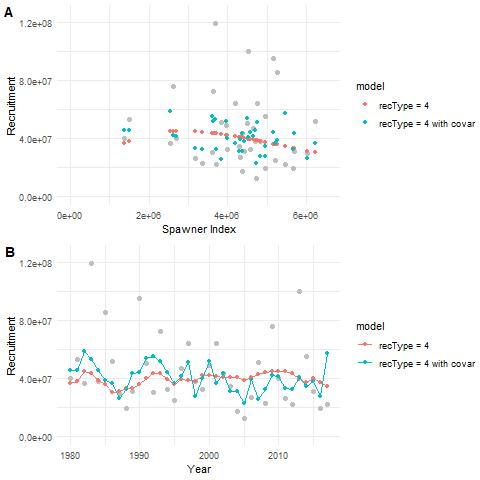
\includegraphics[width=0.8\textwidth,height=\textheight]{../Figs/recplot5.jpg}

\begin{center}\rule{0.5\linewidth}{0.5pt}\end{center}

\hypertarget{running-futr}{%
\section{Running futR()}\label{running-futr}}

\hypertarget{getting-started}{%
\subsection{Getting started}\label{getting-started}}

\hypertarget{step-1-installing-futr}{%
\subsubsection{Step 1: Installing futR()}\label{step-1-installing-futr}}

The package can be installed from github using the devtools package:

\begin{Shaded}
\begin{Highlighting}[]
\FunctionTok{install.packages}\NormalTok{(}\StringTok{"devtools"}\NormalTok{)}
\end{Highlighting}
\end{Shaded}

The projection package can then be installed to R directly:

\begin{Shaded}
\begin{Highlighting}[]
\NormalTok{devtools}\SpecialCharTok{::}\FunctionTok{install\_github}\NormalTok{(}\StringTok{"kholsman/futR"}\NormalTok{)}
\end{Highlighting}
\end{Shaded}

\hypertarget{step-2-set-up-the-workspace}{%
\subsubsection{Step 2: Set up the
workspace}\label{step-2-set-up-the-workspace}}

The base function for fitting recruitment requires a data.frame of
recruitment and spawning biomass:

\begin{Shaded}
\begin{Highlighting}[]
  \CommentTok{\# rm(list=ls()); setwd("/Users/kholsman/Documents/GitHub/futR")}
  \CommentTok{\#\_\_\_\_\_\_\_\_\_\_\_\_\_\_\_\_\_\_\_\_\_\_\_\_\_\_\_\_\_\_\_\_\_\_\_\_\_\_\_\_\_\_\_}
  \CommentTok{\# 1. Set things up}
  \CommentTok{\#\_\_\_\_\_\_\_\_\_\_\_\_\_\_\_\_\_\_\_\_\_\_\_\_\_\_\_\_\_\_\_\_\_\_\_\_\_\_\_\_\_\_\_}
  \CommentTok{\# rm(list=ls()) ; dir()}

  \CommentTok{\# load data, packages, setup, etc.}
  \FunctionTok{source}\NormalTok{(}\StringTok{"R/01\_make.R"}\NormalTok{)}

  \CommentTok{\#\_\_\_\_\_\_\_\_\_\_\_\_\_\_\_\_\_\_\_\_\_\_\_\_\_\_\_\_\_\_\_\_\_\_\_\_\_\_\_\_\_\_\_}
  \CommentTok{\# 2. Compile futR (first time through {-} can skip this step after )}
  \CommentTok{\#\_\_\_\_\_\_\_\_\_\_\_\_\_\_\_\_\_\_\_\_\_\_\_\_\_\_\_\_\_\_\_\_\_\_\_\_\_\_\_\_\_\_\_}

\NormalTok{  recompile\_model }\OtherTok{\textless{}{-}} \ConstantTok{FALSE} \CommentTok{\# to recompile the model set to TRUE}

   \ControlFlowTok{if}\NormalTok{(recompile\_model)\{}
\NormalTok{    wd0 }\OtherTok{\textless{}{-}} \FunctionTok{getwd}\NormalTok{()}
    \FunctionTok{setwd}\NormalTok{(}\StringTok{"src/TMB"}\NormalTok{)}
      \FunctionTok{recompile}\NormalTok{(}\StringTok{\textquotesingle{}futR\textquotesingle{}}\NormalTok{)}
    \FunctionTok{setwd}\NormalTok{(wd0)}
\NormalTok{   \}}
  \CommentTok{\# this will generate warnings {-} they can be ignored if "0" is returned}
\end{Highlighting}
\end{Shaded}

\emph{Note: If you get a compilation error try reinstalling RTools using
the instructions
\href{https://cran.r-project.org/bin/windows/Rtools/}{here}.}

\begin{Shaded}
\begin{Highlighting}[]
 \CommentTok{\# read in the data and create a datlist}
\NormalTok{  datlist }\OtherTok{\textless{}{-}} \FunctionTok{makefutR\_data}\NormalTok{(}\StringTok{"data/in/futR\_Inputs.xlsx"}\NormalTok{ )}
  
  \CommentTok{\# recruitment data:}
\NormalTok{  datlist}\SpecialCharTok{$}\NormalTok{rs\_dat}\SpecialCharTok{$}\NormalTok{R\_obs}
\NormalTok{  datlist}\SpecialCharTok{$}\NormalTok{rs\_dat}\SpecialCharTok{$}\NormalTok{S\_obs}
  
  \CommentTok{\# covar data:}
\NormalTok{  datlist}\SpecialCharTok{$}\NormalTok{rs\_dat}\SpecialCharTok{$}\NormalTok{rs\_cov}
  \CommentTok{\# rec        \textless{}{-}  rec\_dat[[1]]}
  \CommentTok{\# env        \textless{}{-}  env\_covars}

  \CommentTok{\# which parameters to estimate with futR?}
\NormalTok{  datlist}\SpecialCharTok{$}\NormalTok{estparams}
  
  \CommentTok{\# starting values? }
\NormalTok{  datlist}\SpecialCharTok{$}\NormalTok{parameters}
  
  \CommentTok{\# parameter map:}
\NormalTok{  datlist}\SpecialCharTok{$}\NormalTok{maplist}
  
  \CommentTok{\# which phases to estimate in (not yet coded up)}
\NormalTok{  datlist}\SpecialCharTok{$}\NormalTok{phases}

 
  \CommentTok{\# set some global values for the demo below:}
\NormalTok{  estparams }\OtherTok{\textless{}{-}}\NormalTok{  datlist}\SpecialCharTok{$}\NormalTok{estparams[}\DecValTok{1}\SpecialCharTok{:}\DecValTok{6}\NormalTok{]}
\NormalTok{  rec       }\OtherTok{\textless{}{-}}  \FunctionTok{data.frame}\NormalTok{(readxl}\SpecialCharTok{::}\FunctionTok{read\_xlsx}\NormalTok{(}\StringTok{"data/in/futR\_Inputs.xlsx"}\NormalTok{ , }\AttributeTok{sheet =} \StringTok{"rec\_data"}\NormalTok{ ))}
\end{Highlighting}
\end{Shaded}

\hypertarget{explore-recruitment-models}{%
\subsection{Explore recruitment
models}\label{explore-recruitment-models}}

\hypertarget{rectype-1}{%
\subsubsection{rectype = 1}\label{rectype-1}}

Log-linear relationship (mean with variation with covars).
\[ \mathrm{log}(\hat{R_i})= a+\sum_{k=1}^{n_k}{\theta_i^{\beta}\beta_k X_{k,i}}+\varepsilon_i \]

\begin{Shaded}
\begin{Highlighting}[]
  \CommentTok{\# makeDat will make the input values, data, and phases for the model:}
  
  \CommentTok{\# hand code datlist:}
\NormalTok{  datlist  }\OtherTok{\textless{}{-}}  \FunctionTok{makeDat}\NormalTok{(}
                    \AttributeTok{rectype    =}  \DecValTok{1}\NormalTok{,}
                    \AttributeTok{tauIN      =}  \DecValTok{0}\NormalTok{,}
                    \AttributeTok{sigMethod  =}  \DecValTok{1}\NormalTok{, }\CommentTok{\# (default, no random effects)}
                    \AttributeTok{estparams  =}\NormalTok{  estparams,}
                    \AttributeTok{estMode    =}  \DecValTok{1}\NormalTok{,}
                    \AttributeTok{rec\_years  =}\NormalTok{  rec}\SpecialCharTok{$}\NormalTok{rec\_year,}
                    \AttributeTok{Rec        =}\NormalTok{  rec}\SpecialCharTok{$}\NormalTok{Robs,}
                    \AttributeTok{SSB        =}\NormalTok{  rec}\SpecialCharTok{$}\NormalTok{SSB,}
                    \AttributeTok{sdSSB      =}\NormalTok{  rec}\SpecialCharTok{$}\NormalTok{sdSSB,}
                    \AttributeTok{sdRec      =}\NormalTok{  rec}\SpecialCharTok{$}\NormalTok{sdRobs,}
                    \AttributeTok{covars     =}  \ConstantTok{NULL}\NormalTok{,}
                    \AttributeTok{covars\_sd  =}  \ConstantTok{NULL}\NormalTok{)}

  \CommentTok{\# run the basic model}
\NormalTok{  Rec1 }\OtherTok{\textless{}{-}}\NormalTok{  mm }\OtherTok{\textless{}{-}}\FunctionTok{runRecMod}\NormalTok{(}\AttributeTok{dlistIN   =}\NormalTok{ datlist,}
                          \AttributeTok{version   =} \StringTok{\textquotesingle{}futR\textquotesingle{}}\NormalTok{,}
                          \AttributeTok{recompile =} \ConstantTok{FALSE}\NormalTok{,}
                          \AttributeTok{simulate  =} \ConstantTok{TRUE}\NormalTok{,}
                          \AttributeTok{sim\_nitr  =} \DecValTok{1000}\NormalTok{)}
   \CommentTok{\# summarize results}
\NormalTok{  dfR1    }\OtherTok{\textless{}{-}}  \FunctionTok{data.frame}\NormalTok{(}\AttributeTok{model =} \StringTok{"Rec 1"}\NormalTok{,}
                     \AttributeTok{estimate  =} \FunctionTok{as.vector}\NormalTok{(mm}\SpecialCharTok{$}\NormalTok{sim),}
                     \AttributeTok{parameter =} \FunctionTok{names}\NormalTok{( mm}\SpecialCharTok{$}\NormalTok{mle)[}\FunctionTok{row}\NormalTok{(mm}\SpecialCharTok{$}\NormalTok{sim)])}
\NormalTok{  df      }\OtherTok{\textless{}{-}}\NormalTok{ dfR1}
\NormalTok{  r1\_fit  }\OtherTok{\textless{}{-}} \FunctionTok{getFit}\NormalTok{(mm, }\AttributeTok{nm =} \StringTok{"recType = 1"}\NormalTok{)}
\NormalTok{  rec\_fit }\OtherTok{\textless{}{-}}\NormalTok{ r1\_fit}
  \FunctionTok{rm}\NormalTok{(mm)}
  
  \ControlFlowTok{if}\NormalTok{(}\DecValTok{1} \SpecialCharTok{==} \DecValTok{10}\NormalTok{)\{}
   \FunctionTok{print}\NormalTok{(rec\_fit)}
   \FunctionTok{jpeg}\NormalTok{(}\StringTok{"Figs/recplot1.jpg"}\NormalTok{)}
   \FunctionTok{print}\NormalTok{(}\FunctionTok{plot\_rs}\NormalTok{(rec\_fit))}
   \FunctionTok{dev.off}\NormalTok{()}
\NormalTok{  \}}
\end{Highlighting}
\end{Shaded}

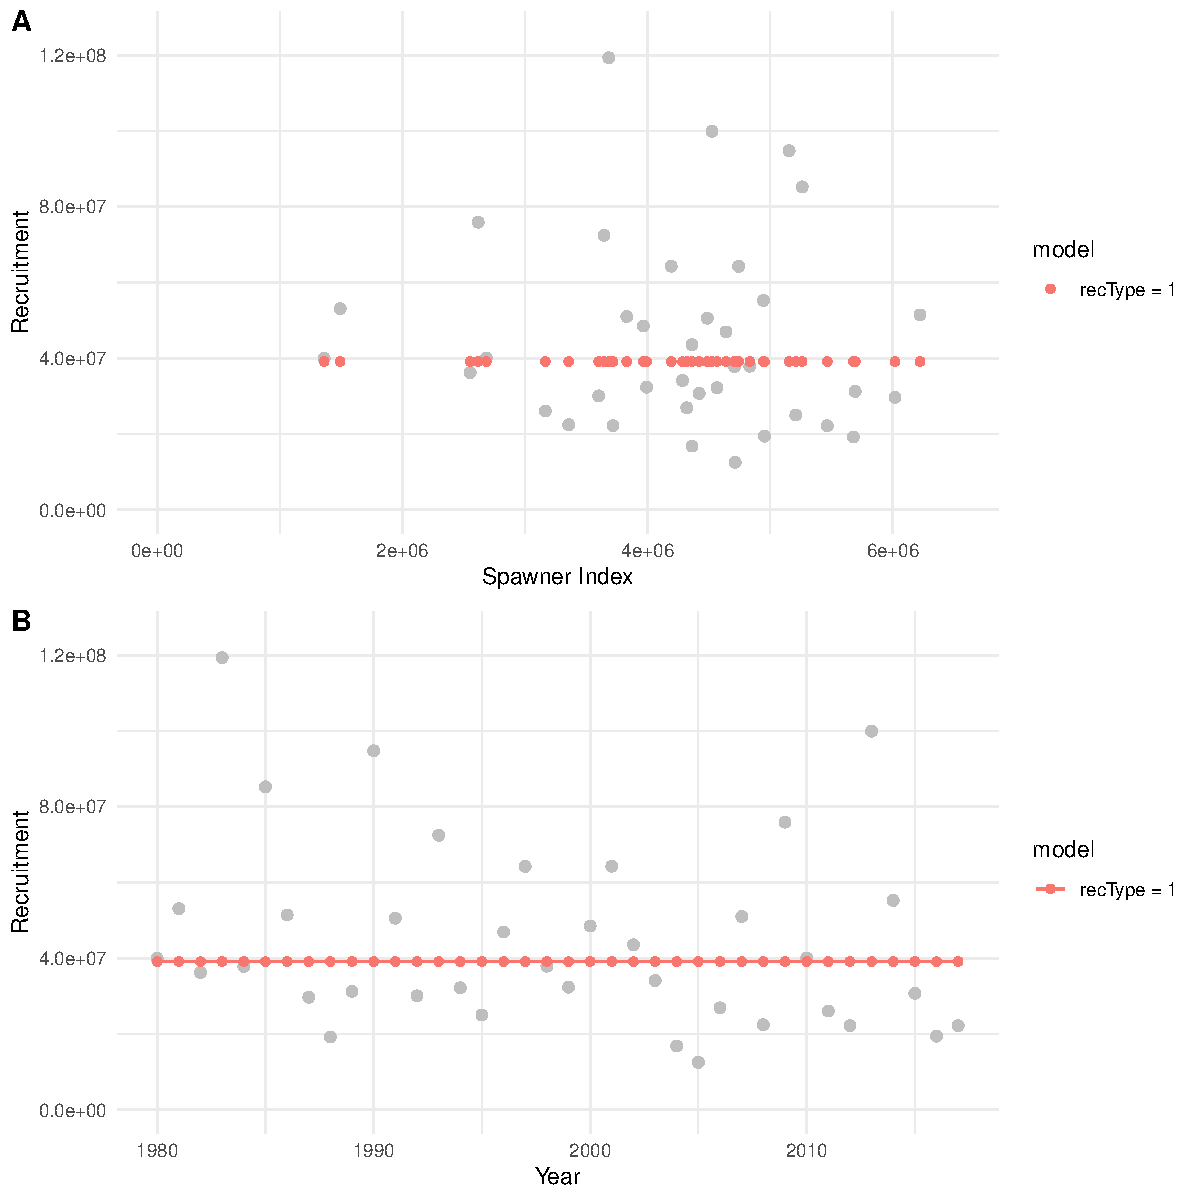
\includegraphics{futR_demo_files/figure-latex/plotR1-1.pdf}

\hypertarget{rectype-2}{%
\subsubsection{rectype = 2}\label{rectype-2}}

Log-linear relationship with spawners and covariates.

\[\mathrm{log}(\hat{R_i})= a + \sum_{k=1}^{n_k}{\theta_i^{\beta}\beta_k X_{k,i}}+ (b+\sum_{k=1}^{n_k}{\theta_i^{\lambda}\lambda_k X_{k,i}})* \hat{S_i}+\varepsilon_i\]

\begin{Shaded}
\begin{Highlighting}[]
  \CommentTok{\# makeDat will make the input values, data, and phases for the model:}
\NormalTok{  estparams1 }\OtherTok{\textless{}{-}}\NormalTok{ estparams}
\NormalTok{  estparams1[}\StringTok{"log\_a"}\NormalTok{] }\OtherTok{\textless{}{-}} \ConstantTok{FALSE}
\NormalTok{  startVal\_1     }\OtherTok{\textless{}{-}}   \FunctionTok{list}\NormalTok{(}\AttributeTok{log\_a =} \SpecialCharTok{{-}}\ConstantTok{Inf}\NormalTok{) }\CommentTok{\# force 0 intercept}
\NormalTok{  datlist  }\OtherTok{\textless{}{-}}  \FunctionTok{makeDat}\NormalTok{(}
                    \AttributeTok{rectype    =}  \DecValTok{2}\NormalTok{,}
                    \AttributeTok{tauIN      =}  \DecValTok{0}\NormalTok{,}
                    \AttributeTok{sigMethod  =}  \DecValTok{1}\NormalTok{, }\CommentTok{\# (default, no random effects)}
                    \AttributeTok{estparams  =}\NormalTok{  estparams1, }\CommentTok{\# set to estparams to allow est of log\_a}
                    \AttributeTok{startVal   =}\NormalTok{  startVal\_1, }\CommentTok{\# set to NULL to remove 0 intercept}
                    \AttributeTok{estMode    =}  \DecValTok{1}\NormalTok{,}
                    \AttributeTok{rec\_years  =}\NormalTok{  rec}\SpecialCharTok{$}\NormalTok{rec\_year,}
                    \AttributeTok{Rec        =}\NormalTok{  rec}\SpecialCharTok{$}\NormalTok{Robs,}
                    \AttributeTok{SSB        =}\NormalTok{  rec}\SpecialCharTok{$}\NormalTok{SSB,}
                    \AttributeTok{sdSSB      =}\NormalTok{  rec}\SpecialCharTok{$}\NormalTok{sdSSB,}
                    \AttributeTok{sdRec      =}\NormalTok{  rec}\SpecialCharTok{$}\NormalTok{sdRobs,}
                    \AttributeTok{covars     =}  \ConstantTok{NULL}\NormalTok{,}
                    \AttributeTok{covars\_sd  =}  \ConstantTok{NULL}\NormalTok{)}

  \CommentTok{\# run the basic model}
\NormalTok{  Rec2 }\OtherTok{\textless{}{-}}\NormalTok{  mm }\OtherTok{\textless{}{-}}\FunctionTok{runRecMod}\NormalTok{(}\AttributeTok{dlistIN   =}\NormalTok{ datlist,}
                          \AttributeTok{version   =} \StringTok{\textquotesingle{}futR\textquotesingle{}}\NormalTok{,}
                          \AttributeTok{recompile =} \ConstantTok{FALSE}\NormalTok{,}
                          \AttributeTok{simulate  =} \ConstantTok{TRUE}\NormalTok{,}
                          \AttributeTok{sim\_nitr  =} \DecValTok{1000}\NormalTok{)}
  \CommentTok{\# summarize results}
\NormalTok{  dfR2    }\OtherTok{\textless{}{-}}  \FunctionTok{data.frame}\NormalTok{(}\AttributeTok{model =} \StringTok{"Rec 2"}\NormalTok{,}
                     \AttributeTok{estimate  =} \FunctionTok{as.vector}\NormalTok{(mm}\SpecialCharTok{$}\NormalTok{sim),}
                     \AttributeTok{parameter =} \FunctionTok{names}\NormalTok{( mm}\SpecialCharTok{$}\NormalTok{mle)[}\FunctionTok{row}\NormalTok{(mm}\SpecialCharTok{$}\NormalTok{sim)])}
\NormalTok{  df      }\OtherTok{\textless{}{-}} \FunctionTok{rbind}\NormalTok{(dfR1,dfR2)}
\NormalTok{  r2\_fit  }\OtherTok{\textless{}{-}} \FunctionTok{getFit}\NormalTok{(mm, }\AttributeTok{nm =} \StringTok{"recType = 2"}\NormalTok{)}
\NormalTok{  rec\_fit }\OtherTok{\textless{}{-}} \FunctionTok{rbind}\NormalTok{(rec\_fit,r2\_fit)}
 \FunctionTok{rm}\NormalTok{(mm)}
 \ControlFlowTok{if}\NormalTok{(}\DecValTok{1}\SpecialCharTok{==}\DecValTok{10}\NormalTok{)\{}
   \FunctionTok{jpeg}\NormalTok{(}\StringTok{"Figs/recplot2.jpg"}\NormalTok{)}
   \FunctionTok{print}\NormalTok{(}\FunctionTok{plot\_rs}\NormalTok{(rec\_fit))}
   \FunctionTok{dev.off}\NormalTok{()}
\NormalTok{ \}}
\end{Highlighting}
\end{Shaded}

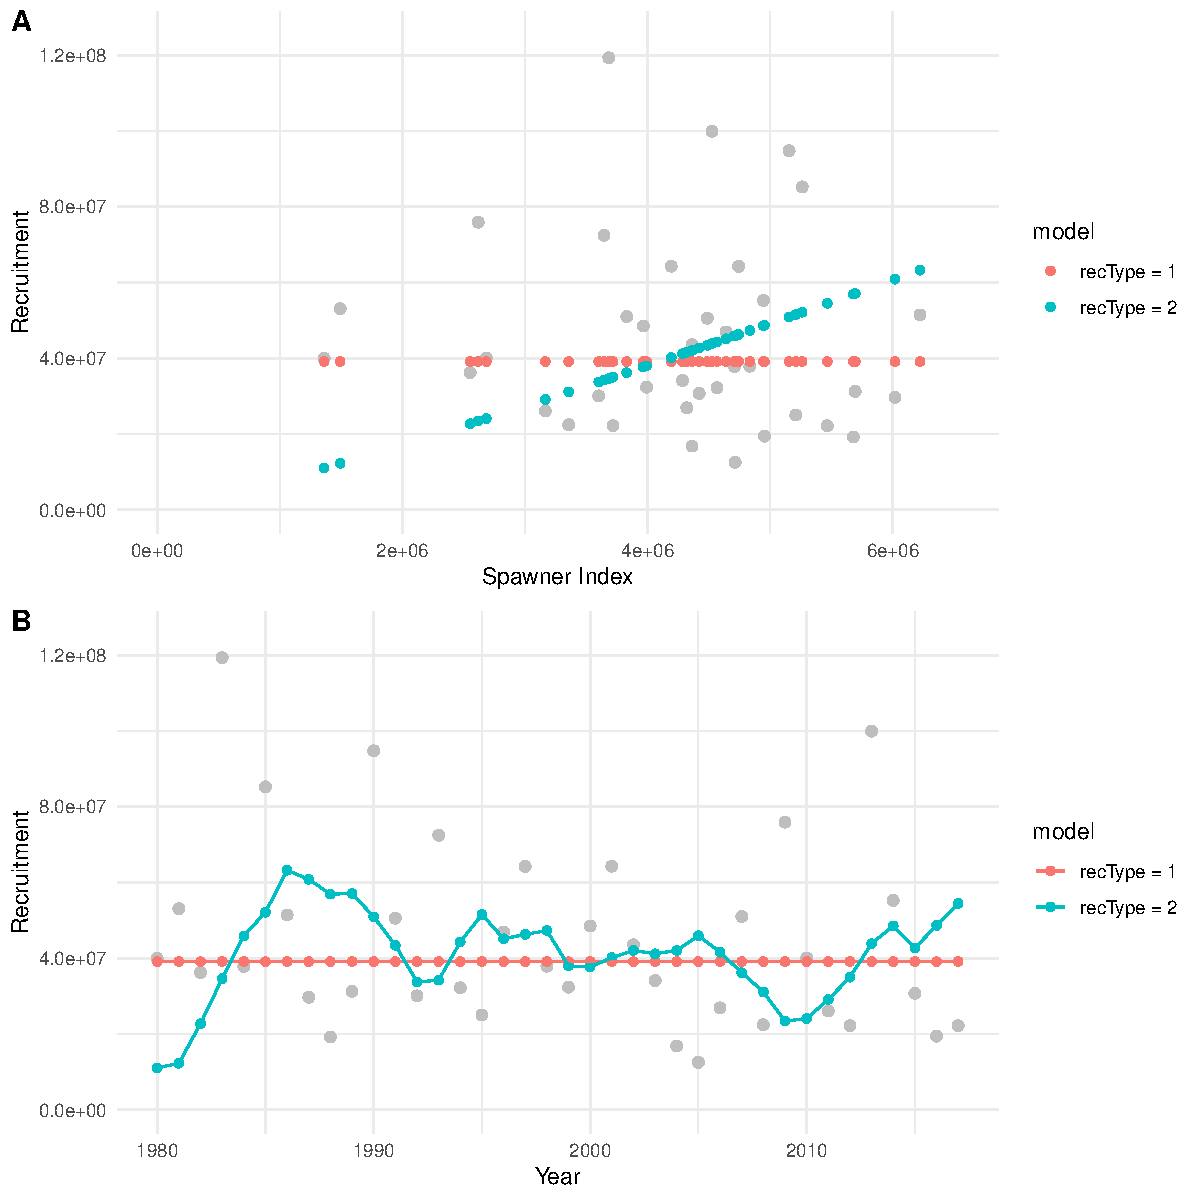
\includegraphics{futR_demo_files/figure-latex/plotR2-1.pdf}

\hypertarget{rectype-3}{%
\subsubsection{rectype = 3}\label{rectype-3}}

Beverton holt relationship.

\[\hat{R_i}=\frac{ a \hat{S_i}e^{ \left( \sum_{k=1}^{n_k}{\theta_i^{\beta}\beta_k X_{k,i}} \right)}}{ 1+b\hat{S_i}e^{\left( \sum_{k=1}^{n_k}{\theta_i^{\lambda}\lambda_k X_{k,i}} \right) }}+e^{\varepsilon_i}\]

\begin{Shaded}
\begin{Highlighting}[]
  \CommentTok{\# makeDat will make the input values, data, and phases for the model:}
\NormalTok{  datlist  }\OtherTok{\textless{}{-}}  \FunctionTok{makeDat}\NormalTok{(}
                    \AttributeTok{rectype    =}  \DecValTok{3}\NormalTok{,}
                    \AttributeTok{tauIN      =}  \DecValTok{0}\NormalTok{,}
                    \AttributeTok{sigMethod  =}  \DecValTok{1}\NormalTok{, }\CommentTok{\# (default, no random effects)}
                    \AttributeTok{estparams  =}\NormalTok{  estparams,}
                    \AttributeTok{estMode    =}  \DecValTok{1}\NormalTok{,}
                    \AttributeTok{rec\_years  =}\NormalTok{  rec}\SpecialCharTok{$}\NormalTok{rec\_year,}
                    \AttributeTok{Rec        =}\NormalTok{  rec}\SpecialCharTok{$}\NormalTok{Robs,}
                    \AttributeTok{SSB        =}\NormalTok{  rec}\SpecialCharTok{$}\NormalTok{SSB,}
                    \AttributeTok{sdSSB      =}\NormalTok{  rec}\SpecialCharTok{$}\NormalTok{sdSSB,}
                    \AttributeTok{sdRec      =}\NormalTok{  rec}\SpecialCharTok{$}\NormalTok{sdRobs,}
                    \AttributeTok{covars     =}  \ConstantTok{NULL}\NormalTok{,}
                    \AttributeTok{covars\_sd  =}  \ConstantTok{NULL}\NormalTok{)}

  \CommentTok{\# run the basic model}
\NormalTok{  Rec3 }\OtherTok{\textless{}{-}}\NormalTok{  mm }\OtherTok{\textless{}{-}}\FunctionTok{runRecMod}\NormalTok{(}\AttributeTok{dlistIN   =}\NormalTok{ datlist,}
                          \AttributeTok{version   =} \StringTok{\textquotesingle{}futR\textquotesingle{}}\NormalTok{,}
                          \AttributeTok{recompile =} \ConstantTok{FALSE}\NormalTok{,}
                          \AttributeTok{simulate  =} \ConstantTok{TRUE}\NormalTok{,}
                          \AttributeTok{sim\_nitr  =} \DecValTok{1000}\NormalTok{)}
  \CommentTok{\# summarize results}
\NormalTok{  dfR3    }\OtherTok{\textless{}{-}}  \FunctionTok{data.frame}\NormalTok{(}\AttributeTok{model =} \StringTok{"Rec 3"}\NormalTok{,}
                     \AttributeTok{estimate  =} \FunctionTok{as.vector}\NormalTok{(mm}\SpecialCharTok{$}\NormalTok{sim),}
                     \AttributeTok{parameter =} \FunctionTok{names}\NormalTok{( mm}\SpecialCharTok{$}\NormalTok{mle)[}\FunctionTok{row}\NormalTok{(mm}\SpecialCharTok{$}\NormalTok{sim)])}
\NormalTok{  df      }\OtherTok{\textless{}{-}} \FunctionTok{rbind}\NormalTok{(df,dfR3)}
\NormalTok{  r3\_fit  }\OtherTok{\textless{}{-}} \FunctionTok{getFit}\NormalTok{(mm, }\AttributeTok{nm =} \StringTok{"recType = 3"}\NormalTok{)}
\NormalTok{  rec\_fit }\OtherTok{\textless{}{-}} \FunctionTok{rbind}\NormalTok{(rec\_fit,r3\_fit)}
  \FunctionTok{rm}\NormalTok{(mm)}
  
  \ControlFlowTok{if}\NormalTok{(}\DecValTok{1}\SpecialCharTok{==}\DecValTok{10}\NormalTok{)\{}
     \FunctionTok{jpeg}\NormalTok{(}\StringTok{"Figs/recplot3.jpg"}\NormalTok{)}
     \FunctionTok{print}\NormalTok{(}\FunctionTok{plot\_rs}\NormalTok{(rec\_fit))}
     \FunctionTok{dev.off}\NormalTok{()}
\NormalTok{  \}}
\end{Highlighting}
\end{Shaded}

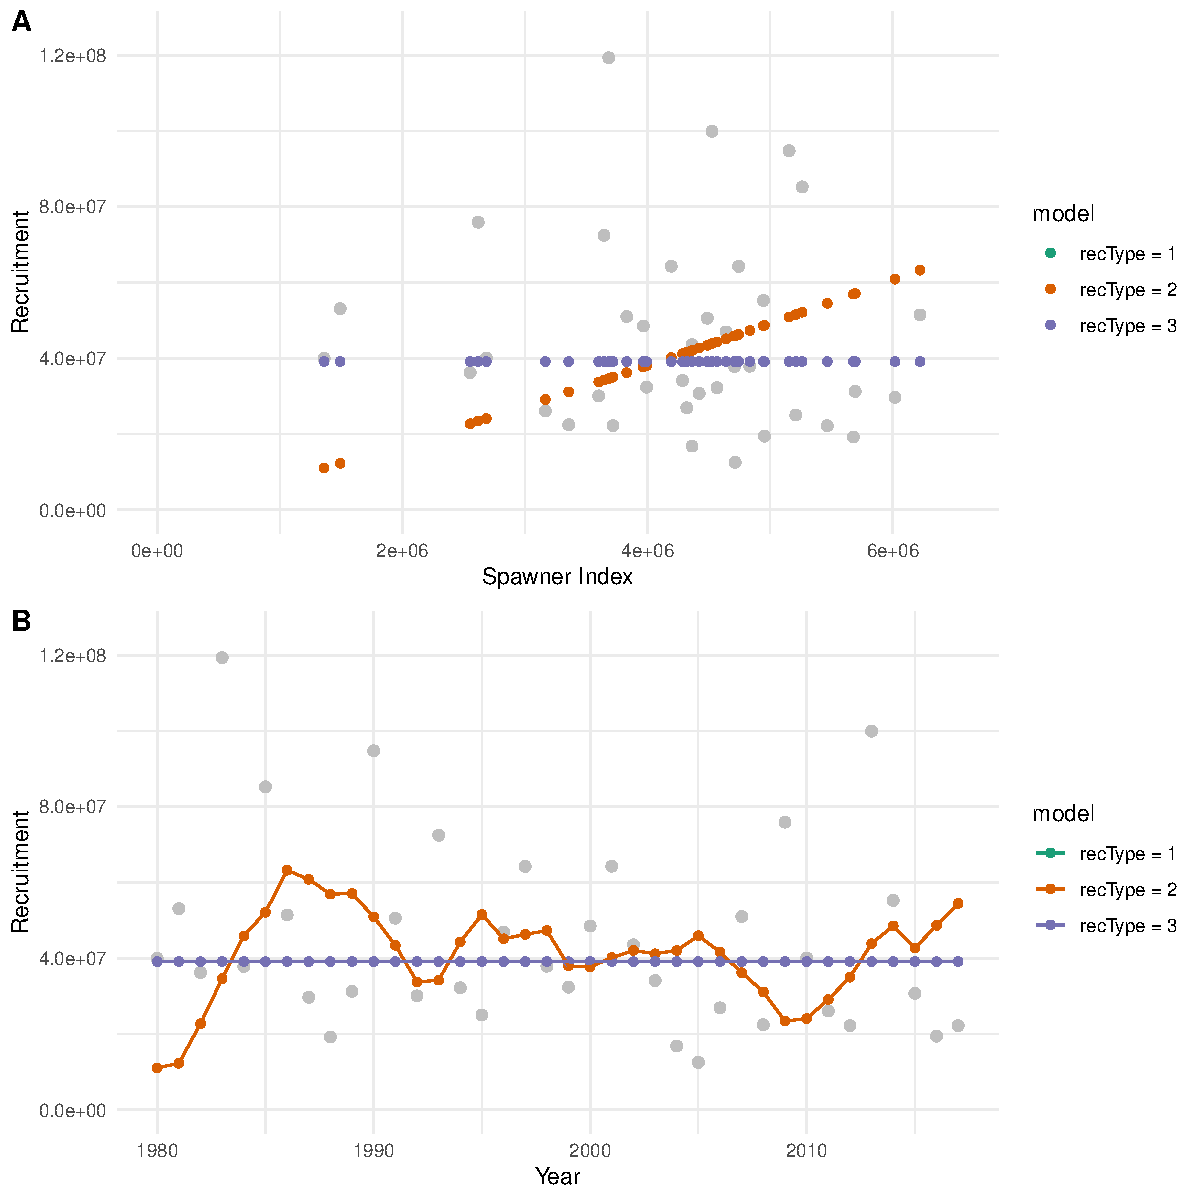
\includegraphics{futR_demo_files/figure-latex/plotR3-1.pdf}

\hypertarget{rectype-4}{%
\subsubsection{rectype = 4}\label{rectype-4}}

Ricker relationship.

\[\mathrm{log}\hat{R_i}= a\left( \sum_{k=1}^{n_k}{\theta_i^{\beta}\beta_k X_{k,i}} \right)-b\hat{S_i}\sum_{k=1}^{n_k}{\theta_i^{\lambda}\lambda_k X_{k,i}}+\hat{S_i}+\varepsilon_i \]

\begin{Shaded}
\begin{Highlighting}[]
  \CommentTok{\# makeDat will make the input values, data, and phases for the model:}
\NormalTok{  datlist  }\OtherTok{\textless{}{-}}  \FunctionTok{makeDat}\NormalTok{(}
                    \AttributeTok{rectype    =}  \DecValTok{4}\NormalTok{,}
                    \AttributeTok{tauIN      =}  \DecValTok{0}\NormalTok{,}
                    \AttributeTok{sigMethod  =}  \DecValTok{1}\NormalTok{, }\CommentTok{\# (default, no random effects)}
                    \AttributeTok{estparams  =}\NormalTok{  estparams,}
                    \AttributeTok{estMode    =}  \DecValTok{1}\NormalTok{,}
                    \AttributeTok{rec\_years  =}\NormalTok{  rec}\SpecialCharTok{$}\NormalTok{rec\_year,}
                    \AttributeTok{Rec        =}\NormalTok{  rec}\SpecialCharTok{$}\NormalTok{Robs,}
                    \AttributeTok{SSB        =}\NormalTok{  rec}\SpecialCharTok{$}\NormalTok{SSB,}
                    \AttributeTok{sdSSB      =}\NormalTok{  rec}\SpecialCharTok{$}\NormalTok{sdSSB,}
                    \AttributeTok{sdRec      =}\NormalTok{  rec}\SpecialCharTok{$}\NormalTok{sdRobs,}
                    \AttributeTok{covars     =}  \ConstantTok{NULL}\NormalTok{,}
                    \AttributeTok{covars\_sd  =}  \ConstantTok{NULL}\NormalTok{)}

  \CommentTok{\# run the basic model}
\NormalTok{  Rec4 }\OtherTok{\textless{}{-}}\NormalTok{  mm }\OtherTok{\textless{}{-}}\FunctionTok{runRecMod}\NormalTok{(}\AttributeTok{dlistIN   =}\NormalTok{ datlist,}
                          \AttributeTok{version   =} \StringTok{\textquotesingle{}futR\textquotesingle{}}\NormalTok{,}
                          \AttributeTok{recompile =} \ConstantTok{FALSE}\NormalTok{,}
                          \AttributeTok{simulate  =} \ConstantTok{TRUE}\NormalTok{,}
                          \AttributeTok{sim\_nitr  =} \DecValTok{1000}\NormalTok{)}

  \CommentTok{\# summarize results}
\NormalTok{  dfR4    }\OtherTok{\textless{}{-}}  \FunctionTok{data.frame}\NormalTok{(}\AttributeTok{model =} \StringTok{"Rec 4"}\NormalTok{,}
                     \AttributeTok{estimate  =} \FunctionTok{as.vector}\NormalTok{(mm}\SpecialCharTok{$}\NormalTok{sim),}
                     \AttributeTok{parameter =} \FunctionTok{names}\NormalTok{( mm}\SpecialCharTok{$}\NormalTok{mle)[}\FunctionTok{row}\NormalTok{(mm}\SpecialCharTok{$}\NormalTok{sim)])}
\NormalTok{  df      }\OtherTok{\textless{}{-}} \FunctionTok{rbind}\NormalTok{(df,dfR3)}
\NormalTok{  r4\_fit  }\OtherTok{\textless{}{-}} \FunctionTok{getFit}\NormalTok{(mm, }\AttributeTok{nm =} \StringTok{"recType = 4"}\NormalTok{)}
\NormalTok{  rec\_fit }\OtherTok{\textless{}{-}} \FunctionTok{rbind}\NormalTok{(rec\_fit,r4\_fit)}
 \FunctionTok{rm}\NormalTok{(mm)}
 \FunctionTok{jpeg}\NormalTok{(}\StringTok{"Figs/recplot4.jpg"}\NormalTok{)}
 \FunctionTok{print}\NormalTok{(}\FunctionTok{plot\_rs}\NormalTok{(rec\_fit))}
 \FunctionTok{dev.off}\NormalTok{()}
\end{Highlighting}
\end{Shaded}

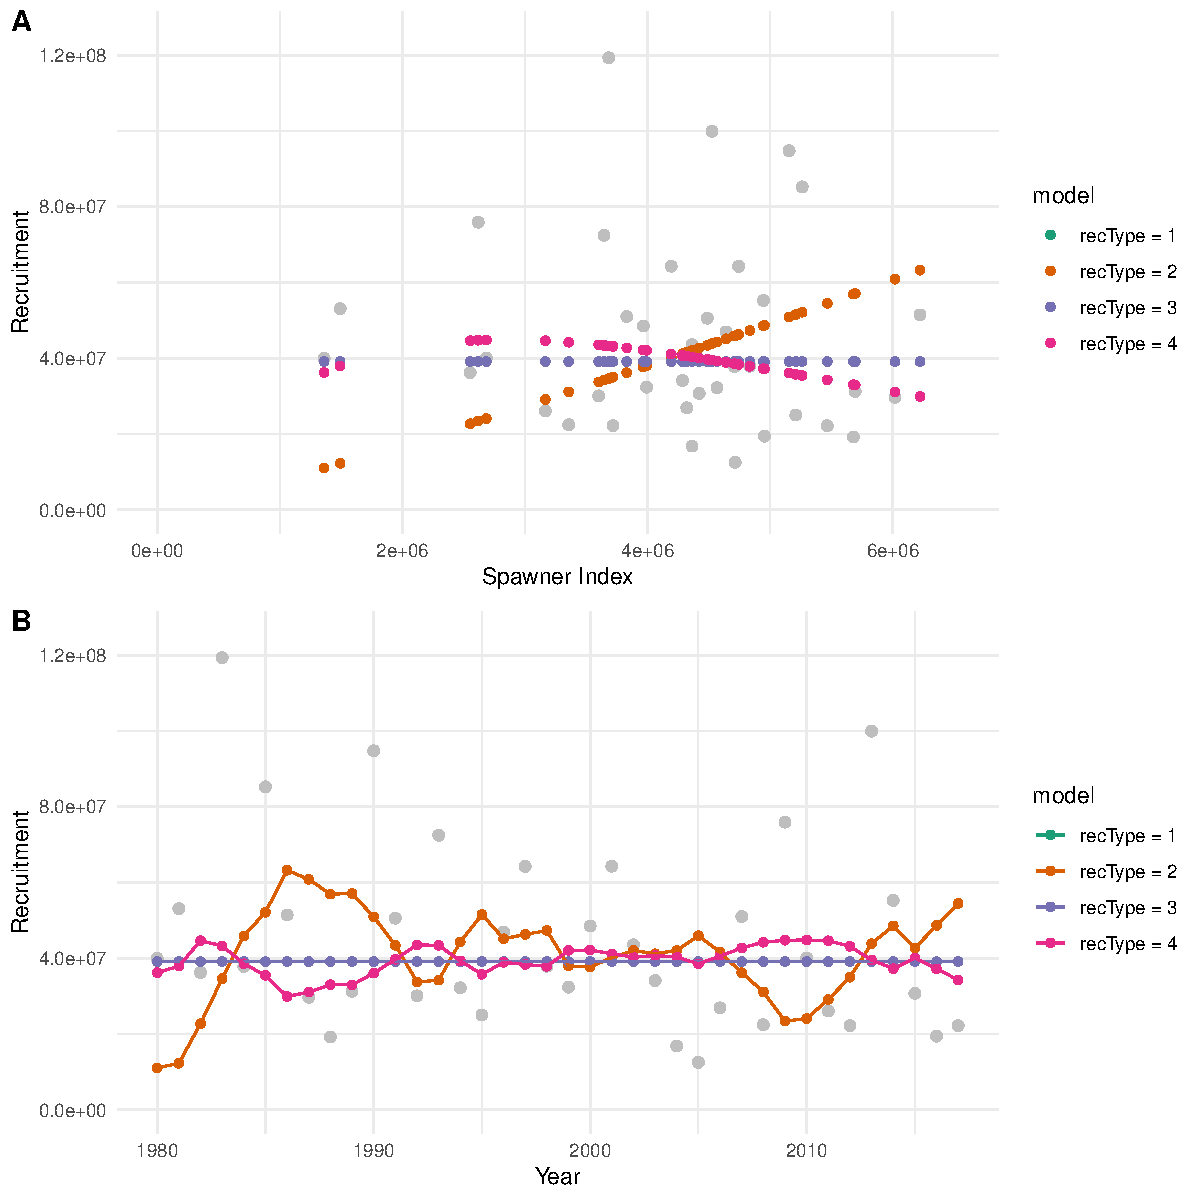
\includegraphics{futR_demo_files/figure-latex/plotR4-1.pdf}

\hypertarget{rectype-4-with-covariates}{%
\subsubsection{rectype = 4 with
covariates}\label{rectype-4-with-covariates}}

Ricker relationship fit with covariates on pre-spawning success and
post-spawning survival.

\[\mathrm{log}\hat{R_i}= a\left( \sum_{k=1}^{n_k}{\theta_i^{\beta}\beta_k X_{k,i}} \right)-b\hat{S_i}\sum_{k=1}^{n_k}{\theta_i^{\lambda}\lambda_k X_{k,i}}+\mathrm{ln}\hat{S_i}+\varepsilon_i \]

\begin{Shaded}
\begin{Highlighting}[]
  \CommentTok{\# read in the data and create a datlist (rather than hand code it)}
\NormalTok{  datlist }\OtherTok{\textless{}{-}} \FunctionTok{makefutR\_data}\NormalTok{(}\StringTok{"data/in/futR\_Inputs.xlsx"}\NormalTok{ )}
  
  
  \CommentTok{\# run the basic model}
\NormalTok{  Rec4\_covar }\OtherTok{\textless{}{-}}\NormalTok{  mm }\OtherTok{\textless{}{-}}\FunctionTok{runRecMod}\NormalTok{(}\AttributeTok{dlistIN   =}\NormalTok{ datlist,}
                          \AttributeTok{version   =} \StringTok{\textquotesingle{}futR\textquotesingle{}}\NormalTok{,}
                          \AttributeTok{recompile =} \ConstantTok{FALSE}\NormalTok{,}
                          \AttributeTok{simulate  =} \ConstantTok{TRUE}\NormalTok{,}
                          \AttributeTok{sim\_nitr  =} \DecValTok{1000}\NormalTok{)}

  \CommentTok{\# summarize results}
\NormalTok{  dfR4\_c    }\OtherTok{\textless{}{-}}  \FunctionTok{data.frame}\NormalTok{(}\AttributeTok{model =} \StringTok{"Rec 4 with covar"}\NormalTok{,}
                     \AttributeTok{estimate  =} \FunctionTok{as.vector}\NormalTok{(mm}\SpecialCharTok{$}\NormalTok{sim),}
                     \AttributeTok{parameter =} \FunctionTok{names}\NormalTok{( mm}\SpecialCharTok{$}\NormalTok{mle)[}\FunctionTok{row}\NormalTok{(mm}\SpecialCharTok{$}\NormalTok{sim)])}
\NormalTok{  df      }\OtherTok{\textless{}{-}} \FunctionTok{rbind}\NormalTok{(dfR4,dfR4\_c)}
\NormalTok{  r4\_fit\_c  }\OtherTok{\textless{}{-}} \FunctionTok{getFit}\NormalTok{(mm, }\AttributeTok{nm =} \StringTok{"recType = 4 with covar"}\NormalTok{)}
\NormalTok{  rec\_fit }\OtherTok{\textless{}{-}} \FunctionTok{rbind}\NormalTok{(r4\_fit,r4\_fit\_c)}
 \FunctionTok{rm}\NormalTok{(mm)}
 \FunctionTok{jpeg}\NormalTok{(}\StringTok{"Figs/recplot5.jpg"}\NormalTok{)}
 \FunctionTok{print}\NormalTok{(}\FunctionTok{plot\_rs}\NormalTok{(rec\_fit))}
 \FunctionTok{dev.off}\NormalTok{()}
\end{Highlighting}
\end{Shaded}

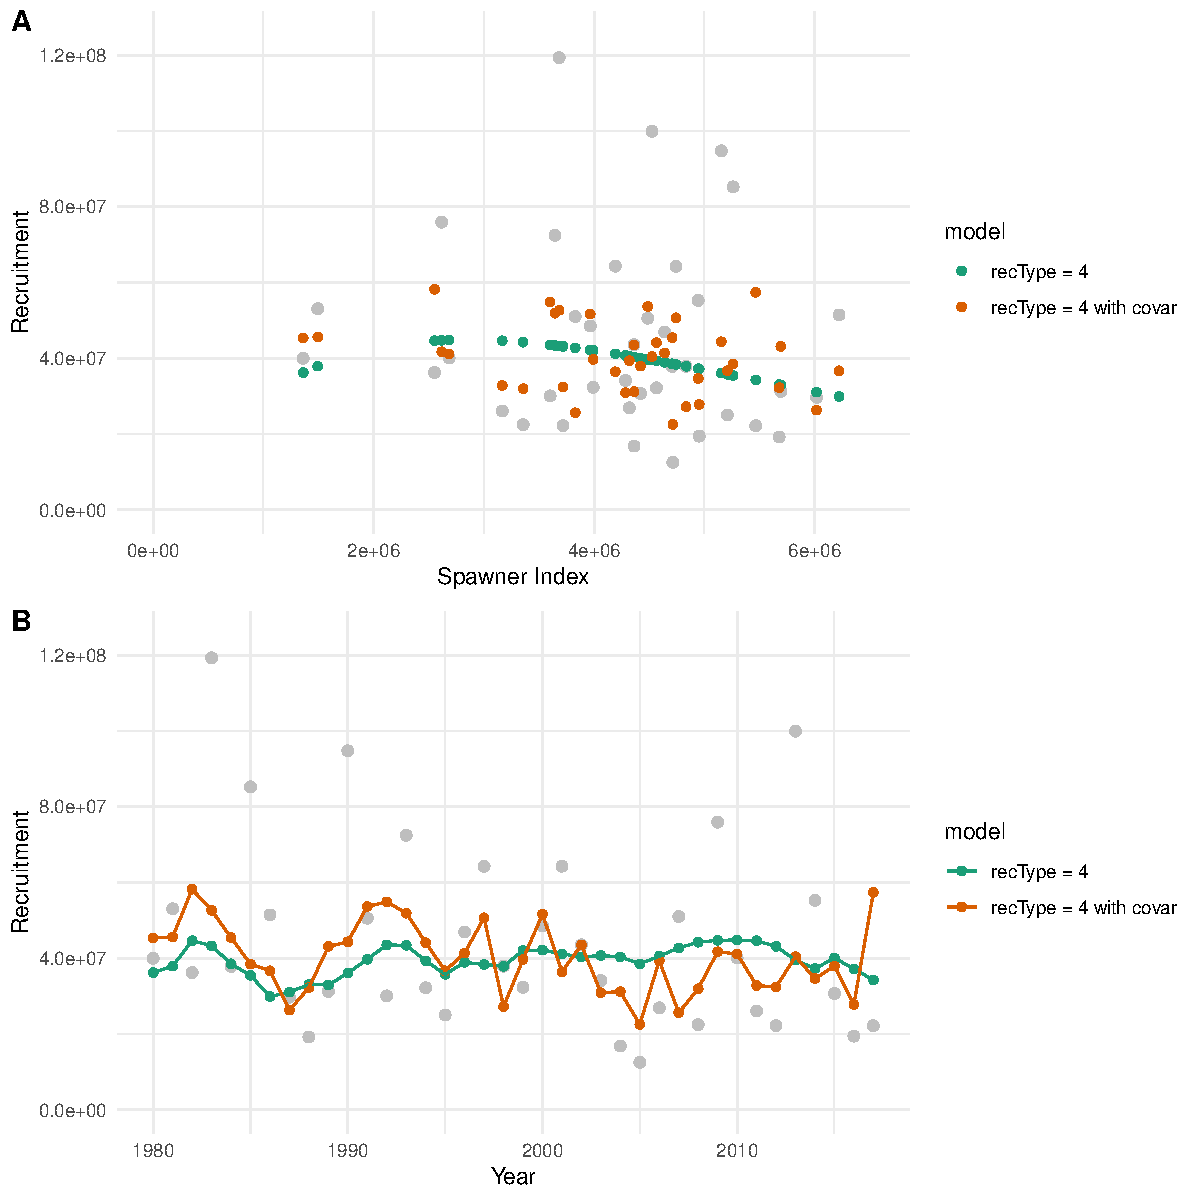
\includegraphics{futR_demo_files/figure-latex/plotR4_cov-1.pdf}

\hypertarget{explore-obs.-error-options}{%
\subsection{Explore obs. error
options}\label{explore-obs.-error-options}}

Let's start by fitting based models (no climate covariates) with
different options for observation error.

\begin{enumerate}
\def\labelenumi{\arabic{enumi}.}
\tightlist
\item
  No observation error (tau = 0)
\item
  estimate sigma, random effects on SSB if tau \textgreater0, tau input
\item
  unbiased sigma estimate, tau input
\item
  as in 1 but with defined measurement error for rec (indep of random
  effects on Spawners/SSB)
\item
  as in 1 but with defined measurement error for rec and Spawners/SSB)
\end{enumerate}

\textbf{Run this code first}

\begin{Shaded}
\begin{Highlighting}[]
\NormalTok{   estparams  }\OtherTok{=} \FunctionTok{c}\NormalTok{(}
    \AttributeTok{log\_a        =} \ConstantTok{TRUE}\NormalTok{,}
    \AttributeTok{log\_b        =} \ConstantTok{TRUE}\NormalTok{,}
    \AttributeTok{beta         =} \ConstantTok{FALSE}\NormalTok{,  }\CommentTok{\# no env covariate}
    \AttributeTok{lambda       =} \ConstantTok{FALSE}\NormalTok{,  }\CommentTok{\# no env covariate}
    \AttributeTok{epsi\_s       =} \ConstantTok{TRUE}\NormalTok{,}
    \AttributeTok{logsigma     =} \ConstantTok{TRUE}\NormalTok{)}

\NormalTok{   rectype\_use }\OtherTok{\textless{}{-}} \DecValTok{4} \CommentTok{\# recType to use (Ricker)}
\end{Highlighting}
\end{Shaded}

Now explore different sigMethod settings starting with sigMethod = 0.
Note comparitive plots at the bottom of each tab.

\hypertarget{sigmethod-1-1}{%
\subsubsection{sigMethod = 1}\label{sigmethod-1-1}}

The base model fits the lognormally distributed process error for
recruitment (\(\sigma\)) using maximum likelihood (i.e., ordinary least
squares). When sigMethod - 0, no observation error (\(\tau = 0\)) is
estimated for either spawners (S) or recruitment (R) estimates.

\begin{Shaded}
\begin{Highlighting}[]
  \CommentTok{\# makeDat will make the input values, data, and phases for the model:}
\NormalTok{  datlist  }\OtherTok{\textless{}{-}}  \FunctionTok{makeDat}\NormalTok{(}
                    \AttributeTok{tauIN      =}  \DecValTok{0}\NormalTok{,  }\CommentTok{\# set tau to zero (no random effects)}
                    \AttributeTok{sigMethod  =}  \DecValTok{1}\NormalTok{,}
                    \AttributeTok{estparams  =}\NormalTok{  estparams,}
                    \AttributeTok{rectype    =}\NormalTok{  rectype\_use, }\CommentTok{\#Ricker}
                    \AttributeTok{rec\_years  =}\NormalTok{  rec}\SpecialCharTok{$}\NormalTok{rec\_year,}
                    \AttributeTok{Rec        =}\NormalTok{  rec}\SpecialCharTok{$}\NormalTok{Robs,}
                    \AttributeTok{SSB        =}\NormalTok{  rec}\SpecialCharTok{$}\NormalTok{SSB,}
                    \AttributeTok{sdSSB      =}\NormalTok{  rec}\SpecialCharTok{$}\NormalTok{sdSSB,}
                    \AttributeTok{sdRec      =}\NormalTok{  rec}\SpecialCharTok{$}\NormalTok{sdRobs,}
                    \AttributeTok{covars     =}  \ConstantTok{NULL}\NormalTok{,}
                    \AttributeTok{covars\_sd  =}  \ConstantTok{NULL}\NormalTok{)}

  \CommentTok{\# run the basic model}

\NormalTok{  m\_S1 }\OtherTok{\textless{}{-}}\NormalTok{  mm }\OtherTok{\textless{}{-}}\FunctionTok{runRecMod}\NormalTok{(}\AttributeTok{dlistIN   =}\NormalTok{ datlist,}
                       \AttributeTok{version   =} \StringTok{\textquotesingle{}futR\textquotesingle{}}\NormalTok{,}
                       \AttributeTok{recompile =}\NormalTok{ F,}
                       \AttributeTok{simulate  =} \ConstantTok{TRUE}\NormalTok{,}
                       \AttributeTok{sim\_nitr  =} \DecValTok{1000}\NormalTok{)}

\NormalTok{  df\_S1 }\OtherTok{\textless{}{-}}  \FunctionTok{data.frame}\NormalTok{(}\AttributeTok{model =} \StringTok{"sigMethod 1"}\NormalTok{,}
                     \AttributeTok{estimate=}\FunctionTok{as.vector}\NormalTok{(mm}\SpecialCharTok{$}\NormalTok{sim),}
                     \AttributeTok{parameter=}\FunctionTok{names}\NormalTok{( mm}\SpecialCharTok{$}\NormalTok{mle)[}\FunctionTok{row}\NormalTok{(mm}\SpecialCharTok{$}\NormalTok{sim)])}
  \FunctionTok{rm}\NormalTok{(mm)}

\NormalTok{  mu   }\OtherTok{\textless{}{-}}\NormalTok{ df\_S1}\SpecialCharTok{\%\textgreater{}\%}\FunctionTok{group\_by}\NormalTok{(model,parameter)}\SpecialCharTok{\%\textgreater{}\%}\FunctionTok{summarise}\NormalTok{(}\AttributeTok{grp.mean=}\FunctionTok{mean}\NormalTok{(estimate))}
\NormalTok{  peak }\OtherTok{\textless{}{-}}\NormalTok{ df\_S1}\SpecialCharTok{\%\textgreater{}\%}\FunctionTok{group\_by}\NormalTok{(model,parameter)}\SpecialCharTok{\%\textgreater{}\%}
    \FunctionTok{count}\NormalTok{(parameter,}\FunctionTok{round}\NormalTok{(estimate,}\DecValTok{1}\NormalTok{))}\SpecialCharTok{\%\textgreater{}\%}
    \FunctionTok{slice}\NormalTok{(}\FunctionTok{which.max}\NormalTok{(n))}
  \FunctionTok{names}\NormalTok{(peak)}\OtherTok{\textless{}{-}} \FunctionTok{c}\NormalTok{(}\StringTok{"model"}\NormalTok{,}\StringTok{"parameter"}\NormalTok{,}\StringTok{"freq"}\NormalTok{,}\StringTok{"n"}\NormalTok{)}
 \FunctionTok{jpeg}\NormalTok{(}\StringTok{"Figs/plotpar1.jpg"}\NormalTok{)}
 \FunctionTok{print}\NormalTok{(}\FunctionTok{plot\_par\_pdf}\NormalTok{(df\_S1))}
 \FunctionTok{dev.off}\NormalTok{()}
\end{Highlighting}
\end{Shaded}

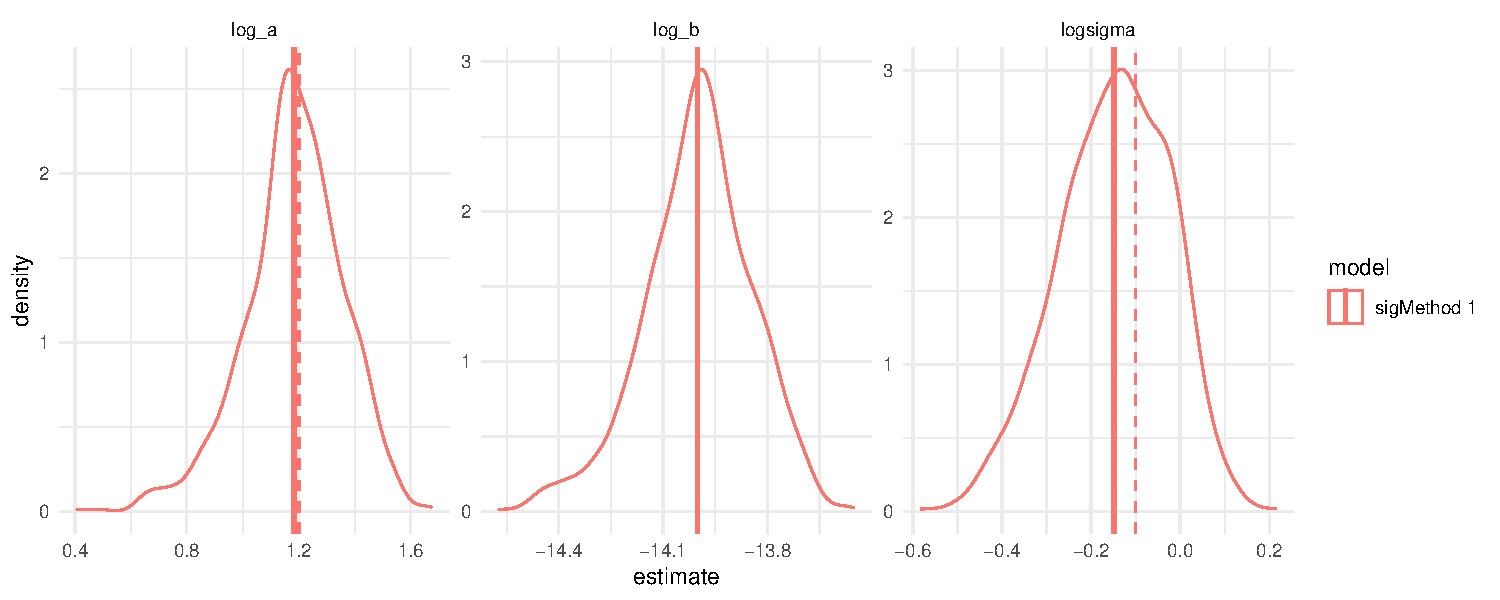
\includegraphics{futR_demo_files/figure-latex/plot1-1.pdf}

\hypertarget{sigmethod-2-1}{%
\subsubsection{sigMethod = 2}\label{sigmethod-2-1}}

The base model fits the lognormally distributed process error for
recruitment (\(\sigma\)) using maximum likelihood (i.e., ordinary least
squares). Additionally, when sigMethod = 1 and \(\tau\) is input
(\(0<\tau<1\)), observation errors are estimated for recruitment and
spawners. Observation errors are statistically independent, random
normal variables with similar variance but because of lack of other
information \(\sigma_R\) is modeled as a function of process error via
the \(\tau\) scalar (see eq 4 in Porch, C. E., and M. V. Lauretta.
2016). Observation error for recruitment is modeled with log-normally
distributed observation error as a function of \(\sigma\) as:
\(log\hat{R}_i\sim N(0,\sigma_R)\) where \(\sigma_R=(1+\tau)*\sigma\)

Similarly, spawner indices (\(\hat{S}_{i-1}\)) include log-normally
distributed observation error as:
\(log\hat{S}_{i-1} \sim N(0,\sigma_S)\) where \(\sigma_S=\tau*\sigma\)

\begin{Shaded}
\begin{Highlighting}[]
  \CommentTok{\# makeDat will make the input values, data, and phases for the model:}
\NormalTok{  datlist  }\OtherTok{\textless{}{-}}  \FunctionTok{makeDat}\NormalTok{(}
                    \AttributeTok{tauIN      =}  \DecValTok{1}\NormalTok{,}
                    \AttributeTok{sigMethod  =}  \DecValTok{2}\NormalTok{,}
                    \AttributeTok{estparams  =}\NormalTok{  estparams,}
                    \AttributeTok{rectype    =}\NormalTok{  rectype\_use, }\CommentTok{\#Ricker}
                    \AttributeTok{rec\_years  =}\NormalTok{  rec}\SpecialCharTok{$}\NormalTok{rec\_year,}
                    \AttributeTok{Rec        =}\NormalTok{  rec}\SpecialCharTok{$}\NormalTok{Robs,}
                    \AttributeTok{SSB        =}\NormalTok{  rec}\SpecialCharTok{$}\NormalTok{SSB,}
                    \AttributeTok{sdSSB      =}\NormalTok{  rec}\SpecialCharTok{$}\NormalTok{sdSSB,}
                    \AttributeTok{sdRec      =}\NormalTok{  rec}\SpecialCharTok{$}\NormalTok{sdRobs,}
                    \AttributeTok{covars     =}  \ConstantTok{NULL}\NormalTok{,}
                    \AttributeTok{covars\_sd  =}  \ConstantTok{NULL}\NormalTok{)}

  \CommentTok{\# re{-}run the model with tau}

\NormalTok{  m\_S2  }\OtherTok{\textless{}{-}}\NormalTok{  mm }\OtherTok{\textless{}{-}}  \FunctionTok{runRecMod}\NormalTok{(}\AttributeTok{dlistIN  =}\NormalTok{ datlist,}
                          \AttributeTok{version  =} \StringTok{\textquotesingle{}futR\textquotesingle{}}\NormalTok{,}
                          \AttributeTok{recompile=}\NormalTok{ F,}
                          \AttributeTok{simulate =} \ConstantTok{TRUE}\NormalTok{,}
                          \AttributeTok{maxitr   =} \DecValTok{100000}\NormalTok{,}
                          \AttributeTok{maxeval  =} \DecValTok{100000}\NormalTok{,}
                          \AttributeTok{sim\_nitr =} \DecValTok{1000}\NormalTok{)}

\NormalTok{  df\_S2 }\OtherTok{\textless{}{-}}  \FunctionTok{data.frame}\NormalTok{(}\AttributeTok{model =} \StringTok{"sigMethod 2"}\NormalTok{,}
                    \AttributeTok{estimate   =} \FunctionTok{as.vector}\NormalTok{(mm}\SpecialCharTok{$}\NormalTok{sim),}
                    \AttributeTok{parameter  =} \FunctionTok{names}\NormalTok{( mm}\SpecialCharTok{$}\NormalTok{mle)[}\FunctionTok{row}\NormalTok{(mm}\SpecialCharTok{$}\NormalTok{sim)])}
  \FunctionTok{rm}\NormalTok{(mm)}
\NormalTok{  df }\OtherTok{\textless{}{-}} \FunctionTok{rbind}\NormalTok{(df\_S1, df\_S2)}
\NormalTok{  mu   }\OtherTok{\textless{}{-}}\NormalTok{ df}\SpecialCharTok{\%\textgreater{}\%}\FunctionTok{group\_by}\NormalTok{(model,parameter)}\SpecialCharTok{\%\textgreater{}\%}\FunctionTok{summarise}\NormalTok{(}\AttributeTok{grp.mean=}\FunctionTok{mean}\NormalTok{(estimate))}
\NormalTok{  peak }\OtherTok{\textless{}{-}}\NormalTok{ df}\SpecialCharTok{\%\textgreater{}\%}\FunctionTok{group\_by}\NormalTok{(model,parameter)}\SpecialCharTok{\%\textgreater{}\%}
    \FunctionTok{count}\NormalTok{(parameter,}\FunctionTok{round}\NormalTok{(estimate,}\DecValTok{1}\NormalTok{))}\SpecialCharTok{\%\textgreater{}\%}
    \FunctionTok{slice}\NormalTok{(}\FunctionTok{which.max}\NormalTok{(n))}
  \FunctionTok{names}\NormalTok{(peak)}\OtherTok{\textless{}{-}} \FunctionTok{c}\NormalTok{(}\StringTok{"model"}\NormalTok{,}\StringTok{"parameter"}\NormalTok{,}\StringTok{"freq"}\NormalTok{,}\StringTok{"n"}\NormalTok{)}
\FunctionTok{jpeg}\NormalTok{(}\StringTok{"Figs/plotpar2.jpg"}\NormalTok{)}
 \FunctionTok{print}\NormalTok{(}\FunctionTok{plot\_par\_pdf}\NormalTok{(df))}
 \FunctionTok{dev.off}\NormalTok{()}
\end{Highlighting}
\end{Shaded}

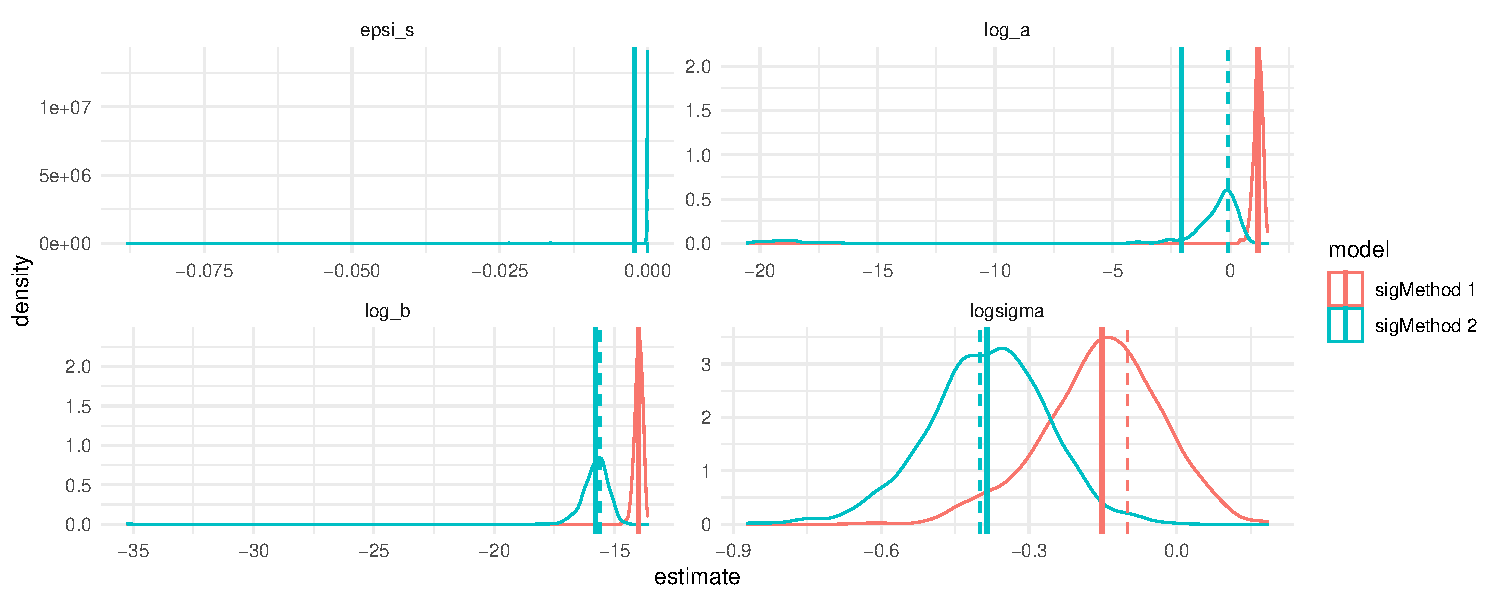
\includegraphics{futR_demo_files/figure-latex/plot2-1.pdf}

\hypertarget{sigmethod-3-1}{%
\subsubsection{sigMethod = 3}\label{sigmethod-3-1}}

As in sigMethod = 2, except when sigMethod = 3 \(\sigma\) is estimated
using the unbiased sigma estimate (sensu Ludwig and Walters 1982):

\[\sigma_i =  \frac1{(n_y-k)}*({ \frac{{\epsilon_{Ri}}^2}{1+\tau} + \frac{{\epsilon_{S,i}}^2}{\tau} })\]
where

\[\epsilon_{Ri} = log(R_i) - log(\hat R_i) \] and
\[\epsilon_{Si} = log(S_i) - log(\hat S_i) \]

\begin{Shaded}
\begin{Highlighting}[]
  \CommentTok{\# makeDat will make the input values, data, and phases for the model:}
\NormalTok{   datlist  }\OtherTok{\textless{}{-}}  \FunctionTok{makeDat}\NormalTok{(}
                    \AttributeTok{tauIN      =}\NormalTok{  .}\DecValTok{001}\NormalTok{,}
                    \AttributeTok{sigMethod  =}  \DecValTok{3}\NormalTok{,}
                    \CommentTok{\#tMethod    =  tm\_use, \#cloglog link (g = 1{-}exp({-}exp(gamma)))}
                    \AttributeTok{estparams  =}\NormalTok{  estparams,}
                    \AttributeTok{rectype    =}\NormalTok{  rectype\_use, }\CommentTok{\#Ricker}
                    \AttributeTok{rec\_years  =}\NormalTok{  rec}\SpecialCharTok{$}\NormalTok{rec\_year,}
                    \AttributeTok{Rec        =}\NormalTok{  rec}\SpecialCharTok{$}\NormalTok{Robs,}
                    \AttributeTok{SSB        =}\NormalTok{  rec}\SpecialCharTok{$}\NormalTok{SSB,}
                    \AttributeTok{sdSSB      =}\NormalTok{  rec}\SpecialCharTok{$}\NormalTok{sdSSB,}
                    \AttributeTok{sdRec      =}\NormalTok{  rec}\SpecialCharTok{$}\NormalTok{sdRobs,}
                    \AttributeTok{covars     =}  \ConstantTok{NULL}\NormalTok{,}
                    \AttributeTok{covars\_sd  =}  \ConstantTok{NULL}\NormalTok{)}


  \CommentTok{\# re{-}run the model with tau}

\NormalTok{  m\_S3 }\OtherTok{\textless{}{-}}\NormalTok{  mm }\OtherTok{\textless{}{-}} \FunctionTok{runRecMod}\NormalTok{(}\AttributeTok{dlistIN   =}\NormalTok{ datlist,}
                        \AttributeTok{version   =} \StringTok{\textquotesingle{}futR\textquotesingle{}}\NormalTok{,}
                        \AttributeTok{recompile =}\NormalTok{ F,}
                        \AttributeTok{simulate  =} \ConstantTok{TRUE}\NormalTok{,}
                        \AttributeTok{sim\_nitr  =} \DecValTok{1000}\NormalTok{)}

\NormalTok{  df\_S3 }\OtherTok{\textless{}{-}}  \FunctionTok{data.frame}\NormalTok{(}\AttributeTok{model =} \StringTok{"sigMethod 3"}\NormalTok{,}
                     \AttributeTok{estimate=}\FunctionTok{as.vector}\NormalTok{(mm}\SpecialCharTok{$}\NormalTok{sim),}
                     \AttributeTok{parameter=}\FunctionTok{names}\NormalTok{( mm}\SpecialCharTok{$}\NormalTok{mle)[}\FunctionTok{row}\NormalTok{(mm}\SpecialCharTok{$}\NormalTok{sim)])}
  \FunctionTok{rm}\NormalTok{(mm)}

\NormalTok{  df }\OtherTok{\textless{}{-}} \FunctionTok{rbind}\NormalTok{(df, df\_S3)}
\NormalTok{  mu   }\OtherTok{\textless{}{-}}\NormalTok{ df}\SpecialCharTok{\%\textgreater{}\%}\FunctionTok{group\_by}\NormalTok{(model,parameter)}\SpecialCharTok{\%\textgreater{}\%}\FunctionTok{summarise}\NormalTok{(}\AttributeTok{grp.mean=}\FunctionTok{mean}\NormalTok{(estimate))}
\NormalTok{  peak }\OtherTok{\textless{}{-}}\NormalTok{ df}\SpecialCharTok{\%\textgreater{}\%}\FunctionTok{group\_by}\NormalTok{(model,parameter)}\SpecialCharTok{\%\textgreater{}\%}
    \FunctionTok{count}\NormalTok{(parameter,}\FunctionTok{round}\NormalTok{(estimate,}\DecValTok{1}\NormalTok{))}\SpecialCharTok{\%\textgreater{}\%}
    \FunctionTok{slice}\NormalTok{(}\FunctionTok{which.max}\NormalTok{(n))}
  \FunctionTok{names}\NormalTok{(peak)}\OtherTok{\textless{}{-}} \FunctionTok{c}\NormalTok{(}\StringTok{"model"}\NormalTok{,}\StringTok{"parameter"}\NormalTok{,}\StringTok{"freq"}\NormalTok{,}\StringTok{"n"}\NormalTok{)}
  \FunctionTok{jpeg}\NormalTok{(}\StringTok{"Figs/plotpar3.jpg"}\NormalTok{)}
  \FunctionTok{print}\NormalTok{(}\FunctionTok{plot\_par\_pdf}\NormalTok{(df))}
  \FunctionTok{dev.off}\NormalTok{()}
\end{Highlighting}
\end{Shaded}

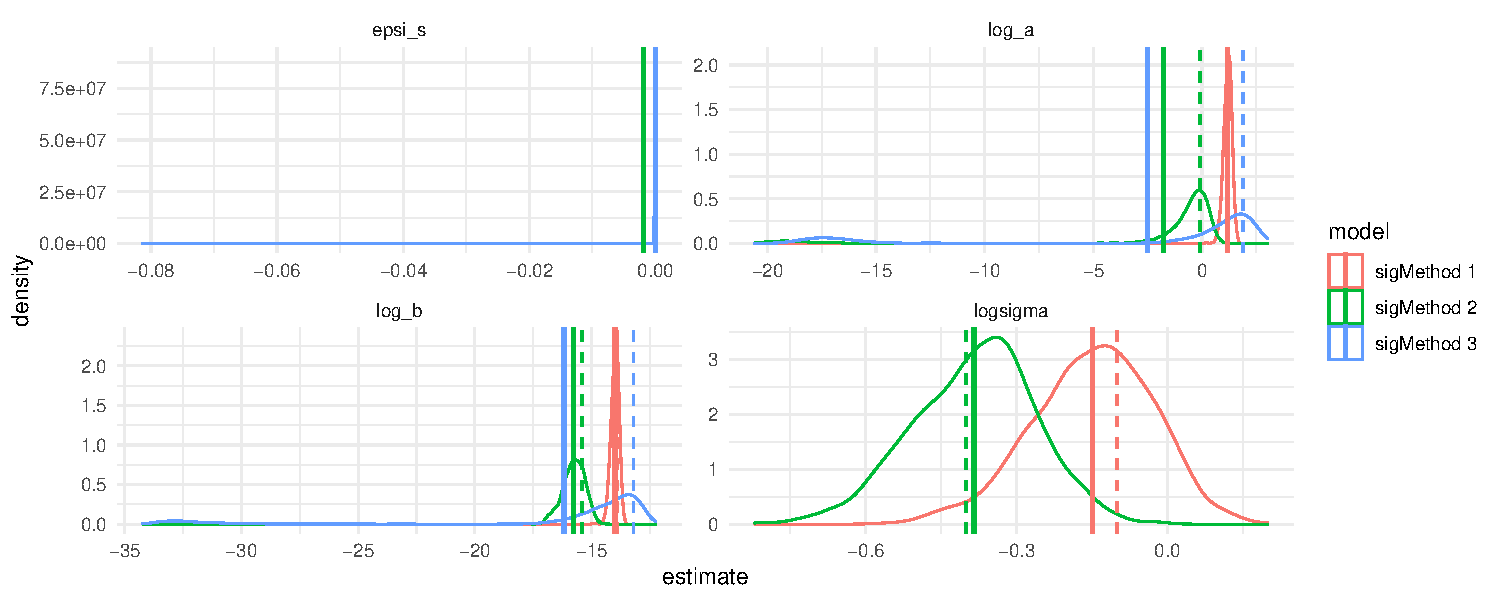
\includegraphics{futR_demo_files/figure-latex/plot3-1.pdf}

\hypertarget{sigmethod-4-1}{%
\subsubsection{sigMethod = 4}\label{sigmethod-4-1}}

As in sigMethod = 2 with observation error (random effects) on S if
\(\tau >0\), but with defined measurement error (\(\gamma_{R,i}\)) for
recruitment estimates (independent of random effects on spawners) such
that:

\(log\hat{R}_i\sim N(0,\sigma_R)\) where
\(\sigma_{R,i}=\sigma_i+\gamma_{R,i}\). and
\(log\hat{S}_{i-1} \sim N(0,\sigma_S\) where \(\sigma_S=\tau*\sigma\).

\begin{Shaded}
\begin{Highlighting}[]
  \CommentTok{\# makeDat will make the input values, data, and phases for the model:}
\NormalTok{   datlist  }\OtherTok{\textless{}{-}}  \FunctionTok{makeDat}\NormalTok{(}
                    \AttributeTok{tauIN      =}\NormalTok{  .}\DecValTok{03}\NormalTok{,}
                    \AttributeTok{sigMethod  =}  \DecValTok{4}\NormalTok{,}
                    \CommentTok{\#tMethod    =  tm\_use, \#cloglog link (g = 1{-}exp({-}exp(gamma)))}
                    \AttributeTok{estparams  =}\NormalTok{  estparams,}
                    \AttributeTok{rectype    =}\NormalTok{  rectype\_use, }\CommentTok{\#Ricker}
                    \AttributeTok{rec\_years  =}\NormalTok{  rec}\SpecialCharTok{$}\NormalTok{rec\_year,}
                    \AttributeTok{Rec        =}\NormalTok{  rec}\SpecialCharTok{$}\NormalTok{Robs,}
                    \AttributeTok{SSB        =}\NormalTok{  rec}\SpecialCharTok{$}\NormalTok{SSB,}
                    \AttributeTok{sdSSB      =}\NormalTok{  rec}\SpecialCharTok{$}\NormalTok{sdSSB,}
                    \AttributeTok{sdRec      =}\NormalTok{  rec}\SpecialCharTok{$}\NormalTok{sdRobs,}
                    \AttributeTok{covars     =}  \ConstantTok{NULL}\NormalTok{,}
                    \AttributeTok{covars\_sd  =}  \ConstantTok{NULL}\NormalTok{)}

  \CommentTok{\# re{-}run the model with tau}
\NormalTok{  m\_S4 }\OtherTok{\textless{}{-}}\NormalTok{  mm }\OtherTok{\textless{}{-}} \FunctionTok{runRecMod}\NormalTok{(}\AttributeTok{dlistIN=}\NormalTok{datlist,}\AttributeTok{version=}\StringTok{\textquotesingle{}futR\textquotesingle{}}\NormalTok{,}\AttributeTok{recompile=}\NormalTok{F,}\AttributeTok{simulate=}\ConstantTok{TRUE}\NormalTok{,}\AttributeTok{sim\_nitr =} \DecValTok{1000}\NormalTok{)}

\NormalTok{  df\_S4 }\OtherTok{\textless{}{-}}  \FunctionTok{data.frame}\NormalTok{(}\AttributeTok{model =} \StringTok{"sigMethod 4"}\NormalTok{,}
                     \AttributeTok{estimate=}\FunctionTok{as.vector}\NormalTok{(mm}\SpecialCharTok{$}\NormalTok{sim),}
                     \AttributeTok{parameter=}\FunctionTok{names}\NormalTok{( mm}\SpecialCharTok{$}\NormalTok{mle)[}\FunctionTok{row}\NormalTok{(mm}\SpecialCharTok{$}\NormalTok{sim)])}
  \FunctionTok{rm}\NormalTok{(mm)}

\NormalTok{  df }\OtherTok{\textless{}{-}} \FunctionTok{rbind}\NormalTok{(df, df\_S4)}
\NormalTok{  mu   }\OtherTok{\textless{}{-}}\NormalTok{ df}\SpecialCharTok{\%\textgreater{}\%}\FunctionTok{group\_by}\NormalTok{(model,parameter)}\SpecialCharTok{\%\textgreater{}\%}\FunctionTok{summarise}\NormalTok{(}\AttributeTok{grp.mean=}\FunctionTok{mean}\NormalTok{(estimate))}
\NormalTok{  peak }\OtherTok{\textless{}{-}}\NormalTok{ df}\SpecialCharTok{\%\textgreater{}\%}\FunctionTok{group\_by}\NormalTok{(model,parameter)}\SpecialCharTok{\%\textgreater{}\%}
    \FunctionTok{count}\NormalTok{(parameter,}\FunctionTok{round}\NormalTok{(estimate,}\DecValTok{1}\NormalTok{))}\SpecialCharTok{\%\textgreater{}\%}
    \FunctionTok{slice}\NormalTok{(}\FunctionTok{which.max}\NormalTok{(n))}
  \FunctionTok{names}\NormalTok{(peak)}\OtherTok{\textless{}{-}} \FunctionTok{c}\NormalTok{(}\StringTok{"model"}\NormalTok{,}\StringTok{"parameter"}\NormalTok{,}\StringTok{"freq"}\NormalTok{,}\StringTok{"n"}\NormalTok{)}
  \FunctionTok{jpeg}\NormalTok{(}\StringTok{"Figs/plotpar4.jpg"}\NormalTok{)}
  \FunctionTok{print}\NormalTok{(}\FunctionTok{plot\_par\_pdf}\NormalTok{(df))}
  \FunctionTok{dev.off}\NormalTok{()}
\end{Highlighting}
\end{Shaded}

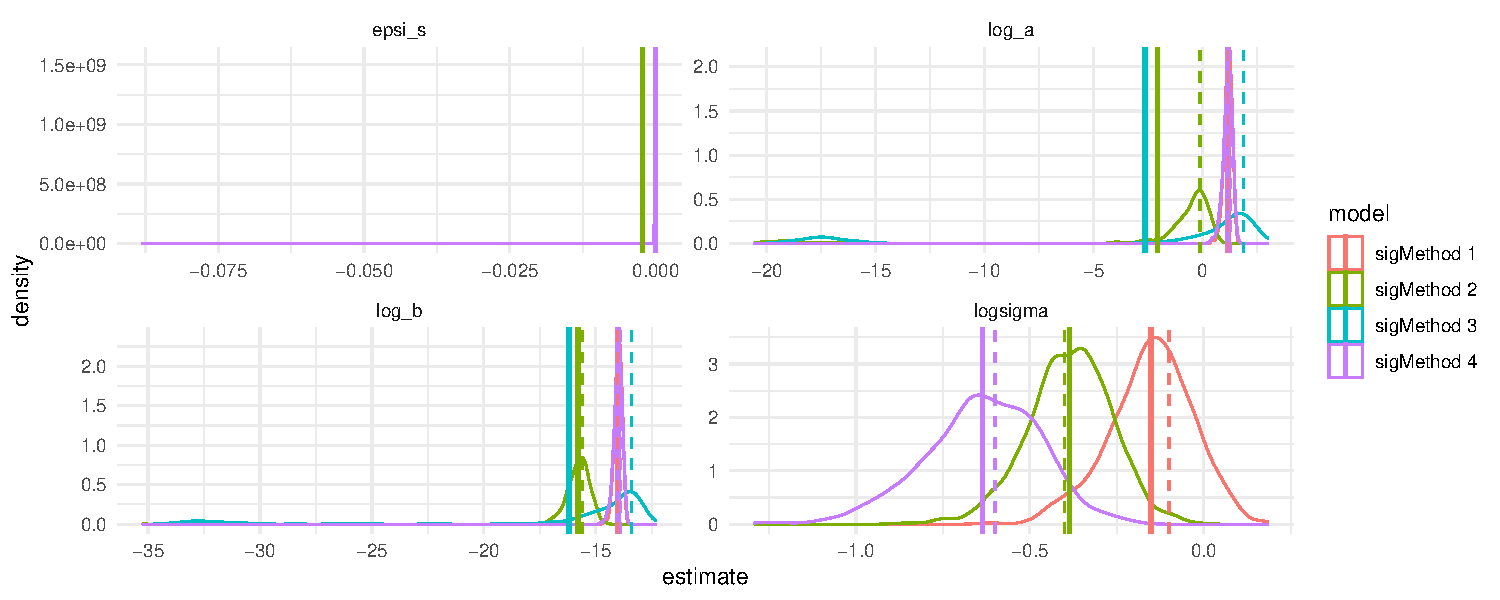
\includegraphics{futR_demo_files/figure-latex/plot4-1.pdf}

\hypertarget{sigmethod-5-1}{%
\subsubsection{sigMethod = 5}\label{sigmethod-5-1}}

As in sigMethod = 2 with observation error (random effects) on S and R
if \(\tau >0\), but with defined measurement errors (\(\gamma_{R,i}\)
and \(\gamma_{S,i}\)) for recruitment and spawner estimates (independent
of random effects on spawners) such that:

\(log\hat{R}_i\sim N(0,\sigma_R)\) where
\(\sigma_{R,i}=((1+\tau)*\sigma_i)+\gamma_{R,i}\). and
\(log\hat{S}_{i-1} \sim N(0,\sigma_S\) where
\(\sigma_S=(\tau*\sigma)+\gamma_{S,i}\).

Note that \(\tau = 0\) defaults to the input variance for S and R as
offsets for each.

\begin{Shaded}
\begin{Highlighting}[]
  \CommentTok{\# makeDat will make the input values, data, and phases for the model:}
\NormalTok{   datlist  }\OtherTok{\textless{}{-}}  \FunctionTok{makeDat}\NormalTok{(}
                    \AttributeTok{tauIN      =}\NormalTok{  .}\DecValTok{03}\NormalTok{,}
                    \AttributeTok{sigMethod  =}  \DecValTok{5}\NormalTok{,}
                    \CommentTok{\#tMethod    =  tm\_use, \#cloglog link (g = 1{-}exp({-}exp(gamma)))}
                    \AttributeTok{estparams  =}\NormalTok{  estparams,}
                    \AttributeTok{rectype    =}\NormalTok{  rectype\_use, }\CommentTok{\#Ricker}
                    \AttributeTok{rec\_years  =}\NormalTok{  rec}\SpecialCharTok{$}\NormalTok{rec\_year,}
                    \AttributeTok{Rec        =}\NormalTok{  rec}\SpecialCharTok{$}\NormalTok{Robs,}
                    \AttributeTok{SSB        =}\NormalTok{  rec}\SpecialCharTok{$}\NormalTok{SSB,}
                    \AttributeTok{sdSSB      =}\NormalTok{  rec}\SpecialCharTok{$}\NormalTok{sdSSB,}
                    \AttributeTok{sdRec      =}\NormalTok{  rec}\SpecialCharTok{$}\NormalTok{sdRobs,}
                    \AttributeTok{covars     =}  \ConstantTok{NULL}\NormalTok{,}
                    \AttributeTok{covars\_sd  =}  \ConstantTok{NULL}\NormalTok{)}


  \CommentTok{\# re{-}run the model with tau}

\NormalTok{  m\_S5 }\OtherTok{\textless{}{-}}\NormalTok{  mm }\OtherTok{\textless{}{-}} \FunctionTok{runRecMod}\NormalTok{(}\AttributeTok{dlistIN=}\NormalTok{datlist,}\AttributeTok{version=}\StringTok{\textquotesingle{}futR\textquotesingle{}}\NormalTok{,}\AttributeTok{recompile=}\NormalTok{F,}\AttributeTok{simulate=}\ConstantTok{TRUE}\NormalTok{,}\AttributeTok{sim\_nitr =} \DecValTok{1000}\NormalTok{)}

\NormalTok{  df\_S5 }\OtherTok{\textless{}{-}}  \FunctionTok{data.frame}\NormalTok{(}\AttributeTok{model =} \StringTok{"sigMethod 5"}\NormalTok{,}
                     \AttributeTok{estimate=}\FunctionTok{as.vector}\NormalTok{(mm}\SpecialCharTok{$}\NormalTok{sim),}
                     \AttributeTok{parameter=}\FunctionTok{names}\NormalTok{( mm}\SpecialCharTok{$}\NormalTok{mle)[}\FunctionTok{row}\NormalTok{(mm}\SpecialCharTok{$}\NormalTok{sim)])}
  \FunctionTok{rm}\NormalTok{(mm)}

\NormalTok{  df }\OtherTok{\textless{}{-}} \FunctionTok{rbind}\NormalTok{(df, df\_S5)}
  \FunctionTok{jpeg}\NormalTok{(}\StringTok{"Figs/plotpar5.jpg"}\NormalTok{)}
 \FunctionTok{print}\NormalTok{(}\FunctionTok{plot\_par\_pdf}\NormalTok{(df))}
 \FunctionTok{dev.off}\NormalTok{()}
\end{Highlighting}
\end{Shaded}

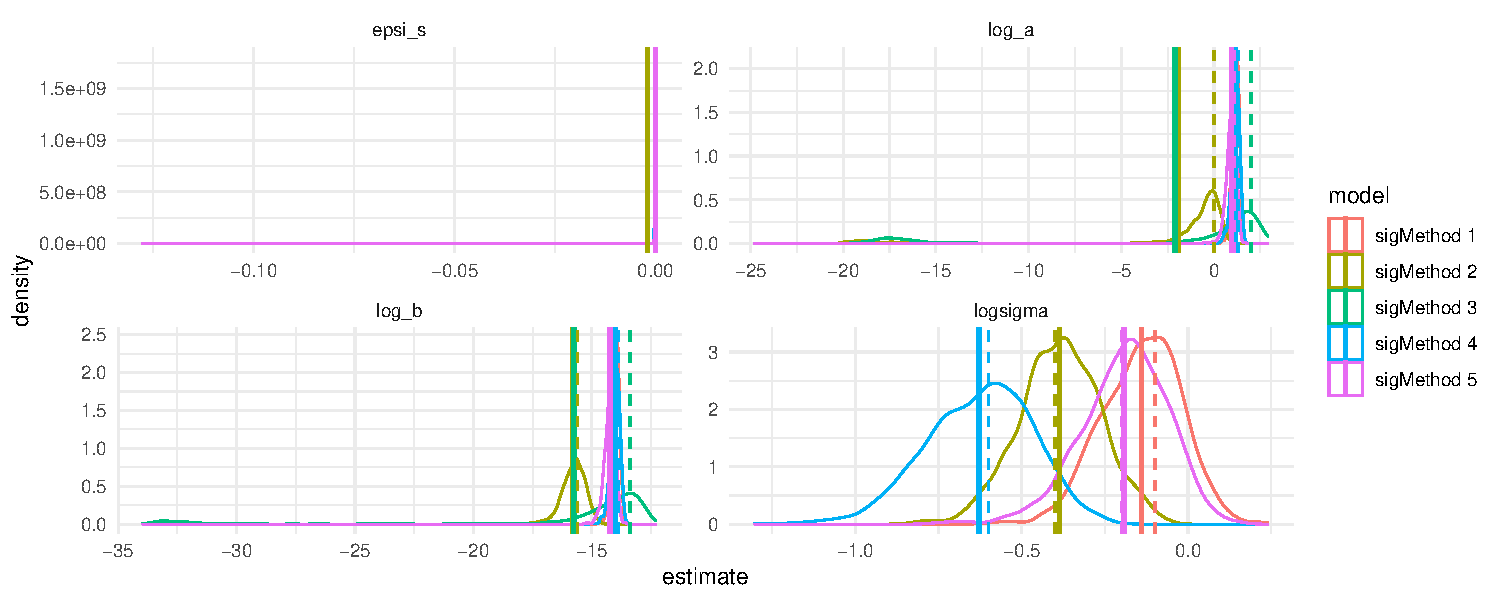
\includegraphics{futR_demo_files/figure-latex/plot5-1.pdf}

\end{document}
